    %\ifx\isEmbedded\undefined
%	% Loading common settings
%	\input{macros/common}
%	% Loading common variable definitions 
%	\input{macros/macros}
%	\begin{document} 
%\else
%\fi
%



\chapter{The Challenge of Vision}
\label{chap:challenge_of_vision}

%In order to write this book, we have adopted the following guideline: if you set up a goal and you fail at it, then just set up another goal. The best way of reaching the finish line is by bringing the finish line to where we are standing. And this is what we did. 

%Our initial goal was to write a large book that provided a good coverage of the field. Unfortunately, the field of computer vision is larger than Texas.  So, we decided to write a small book instead, limiting each chapter to no more than 5 pages. Such a goal forced us to really focus on the important concepts necessary to understand each topic. Unfortunately, we have failed at that too. The result of our failures is this book which, we hope, will motivate you to do better. 

%We believe that this short book is great for the following two reasons: 1) we do not have time to write a long book, and 2) you do not have time to read it. 

\section{Introduction}

%\marginnote{The word "Vision'' has its origin from the word {\em visionem}.}
Let's start with a simple observation: every day, when you wake up, you open your eyes and see. You see without any effort; you do not get tired after a few hours from seeing too much. The same happens with all the other senses. With them you perceive the world around you: you hear the birds or the car noises, you smell the breakfast and feel the touch of the sheets, and that keeps going on and on until the end of the day. But the most surprising fact is that your brain is continuously solving very complex tasks still unmatched by any artificial system. 

The apparent simplicity of perceiving the world around us produces the false intuition that it will be easy to build a machine capable of seeing as humans do. Let's ignore the senses of hearing, touch, taste, and smell, and let's focus on the visual sense. Human vision is capable of extracting information about the world around us using only the light that reflects off surfaces in the direction of our eyes. The light that reaches our eyes does not tell us what object we are looking at. It only give us information about the amount of light reaching our eye from each direction in space. Our brains have to translate the information collected by millions of photoreceptors in our retinas into an interpretation of the world in front of us. What we see is different than the light that reaches our eyes, as visual illusions prove to us.  
\marginnote{This book will focus on the visual sense. Nonetheless, the techniques introduced aren't exclusive to images and possess the versatility to be adapted for the processing of various other signal types.
}

Computer vision studies how to reproduce in a computer the ability to see. Since its origins, the study of vision has been an interdisciplinary study involving many disciplines (physics, psychology, biology, neuroscience, arts, and computer science).

The goal of a vision scientist is twofold: to understand how perception works and to build systems that can interpret the world around them using images (or image sequences) as input. In this chapter, we want to provide a broad perspective on {\bf vision science} and the multiple disciplines that contribute to it.


\section{Vision}

David Marr \cite{Marr82} defines vision as ``to know what is where by looking,'' and  adds ``vision is the process of discovering from images what is present in the world, and where it is.''

It is difficult to say exactly what makes understanding the mechanisms of vision hard as we do not have a full solution yet \cite{Cavanagh96}. In this section we will mention two  aspects that make vision hard: the structure of the input and the structure of the desired output.

What is the goal of vision? Our eyes are sensors, and for an agent that navigates and solves tasks in the world, the role of the sensor is to provide relevant information for solving the task. In the case of computer vision, we mostly study visual perception from a disembodied perspective. There is no agent and there is no task. This perspective makes the study of vision difficult.


\subsection{The Input: The Structure of Ambient Light}

From a light source, a dense array of light rays emerges in all directions. Before these light rays reach the eye, the light interacts with the objects in the world. Let's consider a single ray emerging from the light source (we will use here a simple geometric interpretation of the structure of light). If the light ray is not directed toward the eye, this ray will strike some surface in the world and, as result, a new set of rays will be emitted in many directions. This process will continue producing more and more interactions and filling the space. In the middle of the space the observer will sense only a subset of the light rays that will strike the eye. As a result of this complex pattern of interactions even a single ray will form a complex image in the eye of the observer. 

%Figure~\ref{fig:lightRay} 
\Fig{\ref{fig:lightRay}} shows some pictures taken when illuminating a complex scene with a laser pointer that illuminate the scene with a narrow beam of light (this is the best approximation to the image produced by a single light ray that we could do at home). 

\begin{figure}[t]
\centerline{
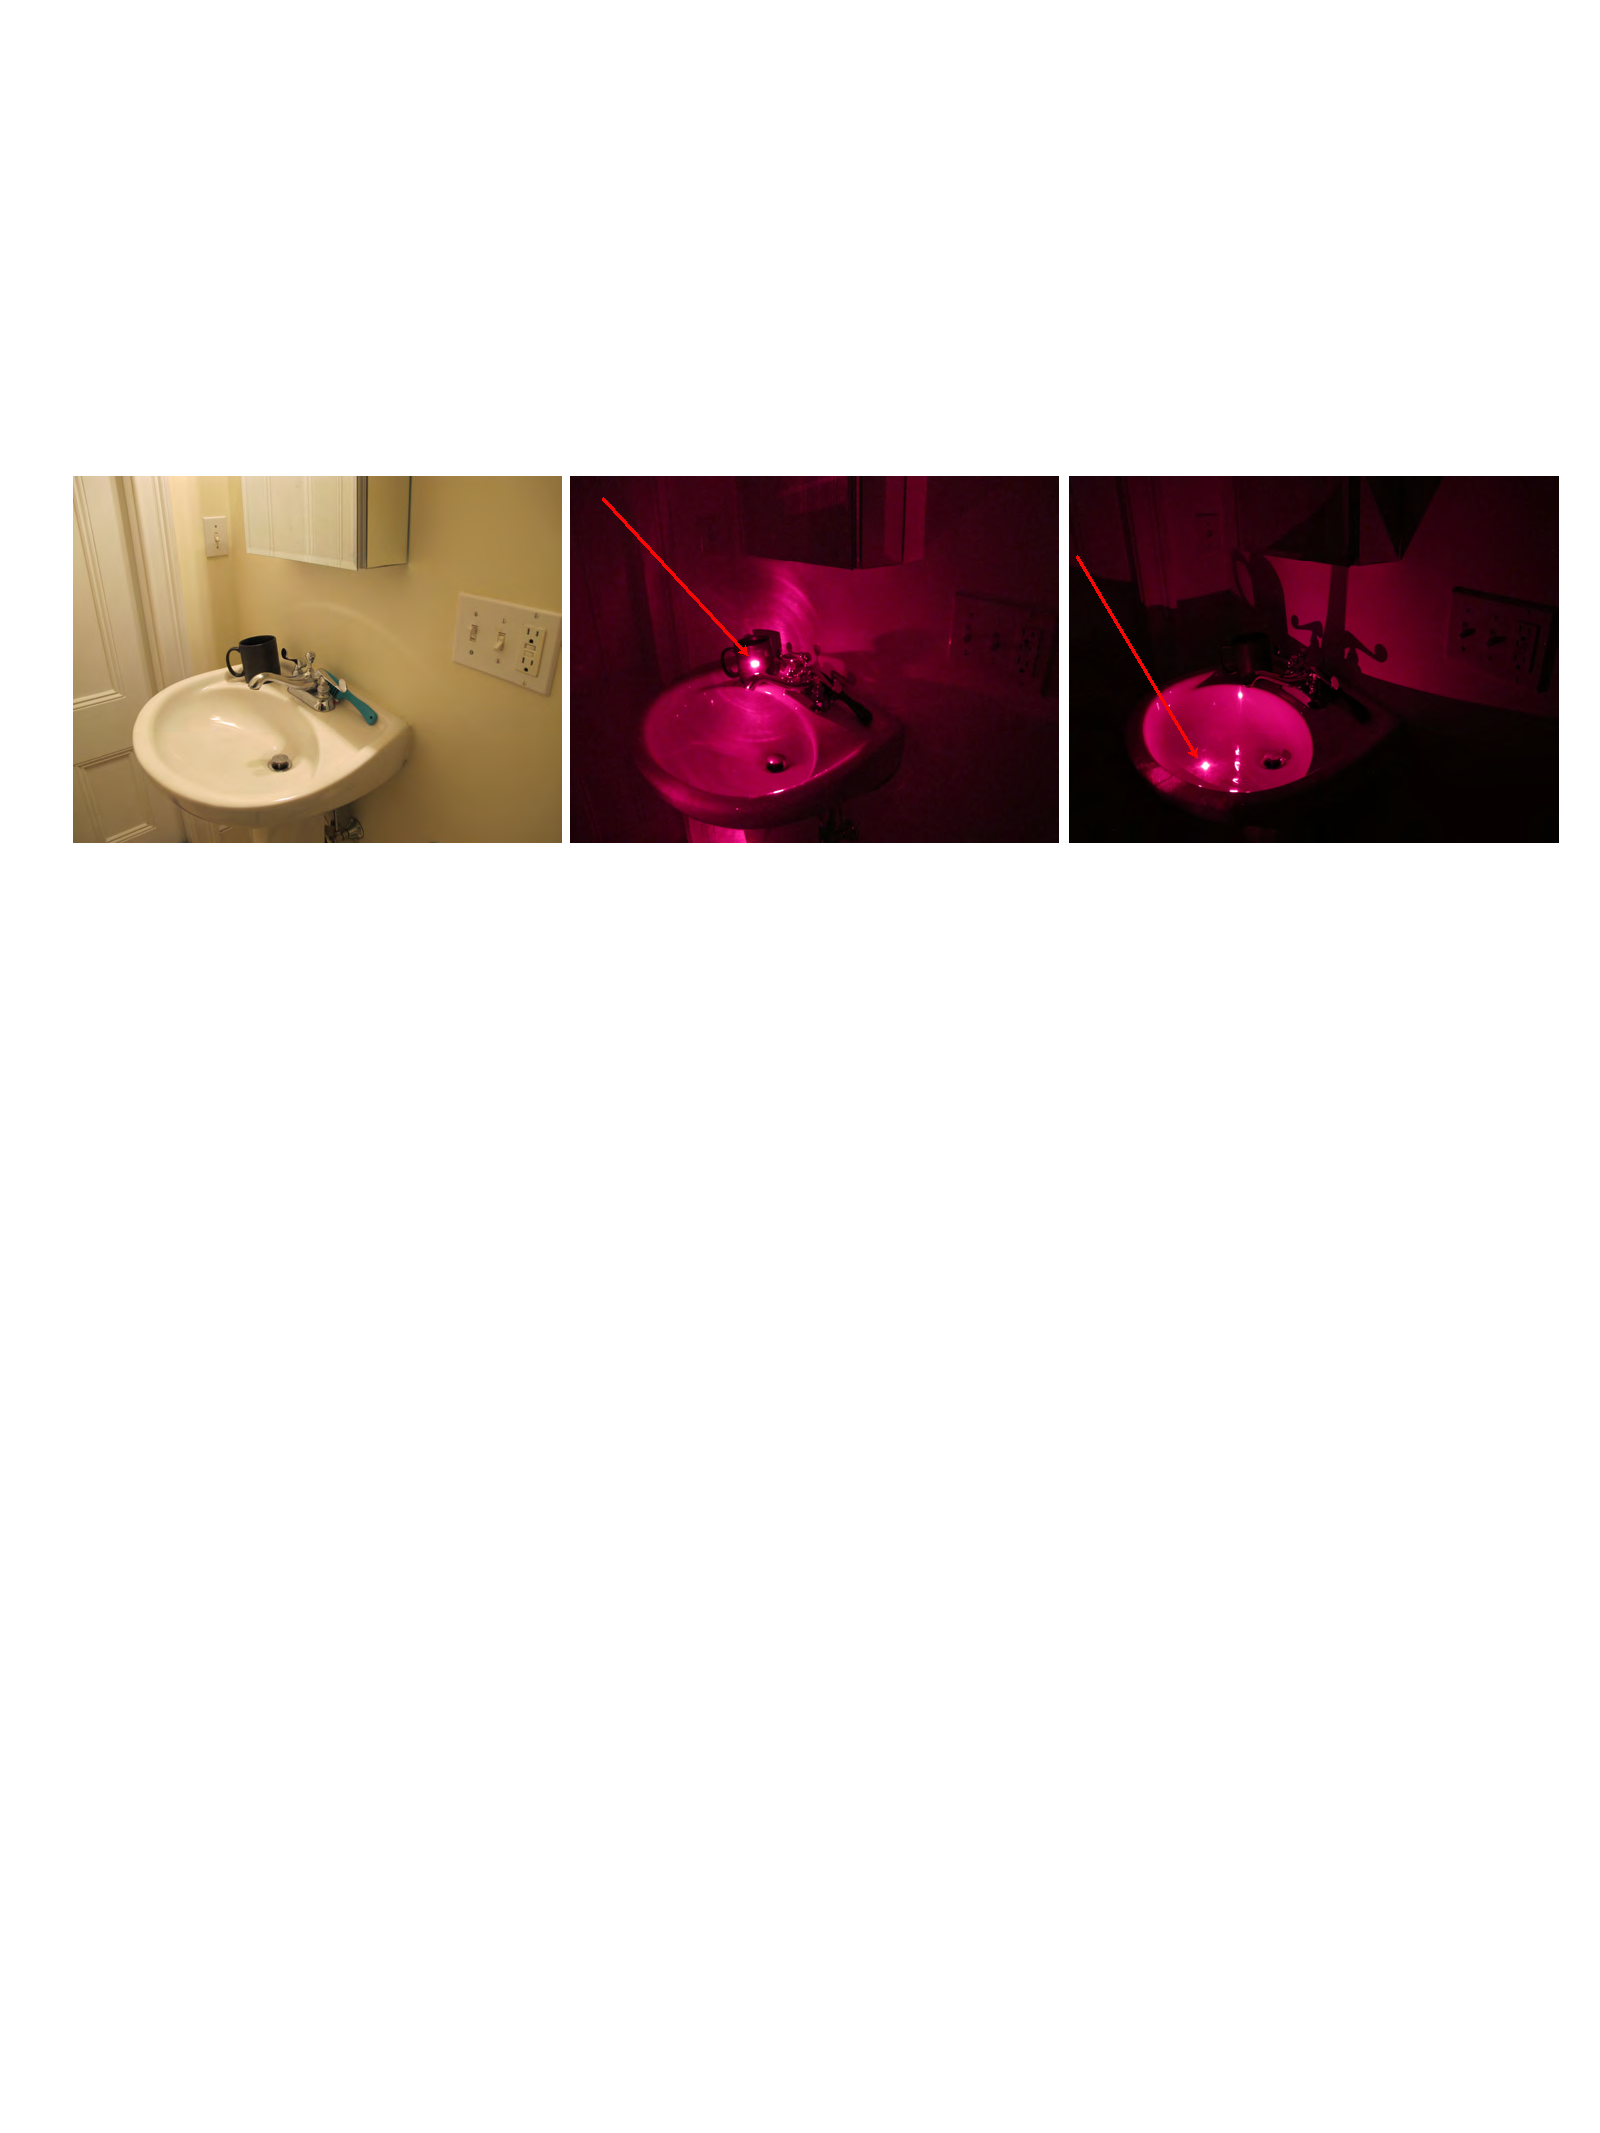
\includegraphics[width=1\linewidth]{figures/taxonomy/lightGray2.pdf}
}
\centerline{
(a)\hspace{1.5in}(b)\hspace{1.5in}(c)
} 
\caption{(a) Scene illuminated with a ceiling lamp. (b-c) Two images obtained by illuminating a scene with a laser pointer (the red line indicates the direction of the ray).} 
\label{fig:lightRay}
\end{figure}

The resulting images show the complexity of the interactions between the different surfaces. The sum of the contribution of all the light rays emitted by the light source will give rise to a natural looking picture. On each image, the approximate direction of the light beam produced by pointer is indicated by the red arrow in \fig{\ref{fig:lightRay}}{b-c}.  

Despite the complexity of the structure of the ambient light (a term coined by James J. Gibson \cite{Gibson1966}) with multiple reflections, shadows, and specular surfaces (which provide incorrect disparity information to our two eyes), our visual system has no problem in interacting with this scene, even if it is among the first things that we see just after waking up. 


The pattern of light filling the space can be described by the function:
\begin{equation}
P (\theta, \Phi, \lambda, t, X, Y, Z)
\end{equation}
%\marginnote{We will study color in \chap{\ref{chapter:color}}.}
where $P$ is the light intensity of a ray passing by the world location $(X,Y,Z)$  in the direction given by the angle $(\theta, \Phi)$, and with wavelength $\lambda$ (we will study color in chapter [\ref{chapter:color}])
%chapter \ref{chapter:color}) 
at an instant in time $t$. This function, called the {\bf plenoptic function} 
\index{Plenoptic function}
Edward H. Adelson  
and James R. Bergen \cite{Adelson91}, contains all the information needed to describe the complete pattern of light rays that fills the space. 
\marginnote{{\bf Plenoptic function}: Edward H. Adelson was going to call it
the {\em holoscopic function}, but a well-known holographer told him that he would punch him in the nose if he called it that.}[.5in]
The plenoptic function does not include information about the observer. The observer does not have access to the entire plenoptic function, only to a small slice of it. In \chap{\ref{chapter:imaging}} we will describe how different mechanisms can produce images by sampling the ambient light in different ways.

For a given observer, most of the light rays are occluded. Without occlusion, vision would be a lot simpler. Occlusion is the best example of how hard vision can get. Many times, properly interpreting an image will require understanding what part is occluded (e.g., we know that a person is not floating just because the legs are occluded behind a table). Unfortunately, occlusions are common. In fact, there are more occluded surfaces than visible surfaces for any given observer.  


Although recovering the entire plenoptic function would have many applications, fortunately, the goal of vision is not to recover this function. 




\subsection{The Output: Measuring Light Versus Measuring Scene Properties}

Vision is not a deterministic process that analyzes the input images independently of our internal state. Even when two people look at the same thing they will have different {\bf visual awareness}. Our visual experience is greatly influenced by what we know, what we are doing, and what we expect to see. 

If the goal vision were  simply to measure the light intensity coming from a particular direction of space (like a photometer) then things would be easy. However, the goal of vision is to provide an interpretation of the world in terms of ``meaningful'' surfaces, objects, materials, etc., in order to extract all the different elements that compose the scene (anything that will be relevant to the observer). This problem is hard because most of the information is lost and the visual system needs to make a number of assumptions about the structure of the visual world in order to be able to recover the desired information from a small sample of the plenoptic function. It is also hard because our understanding about what is relevant for the observer is incomplete. 

The goal of vision is not to measure light intensities, but to extract scene properties relevant for the observer. \Fig{\ref{fig:measuringScene}} shows different images that illustrate that the human visual system is trying to recover the scenes that are the cause of those images. 


\begin{figure}[t]
\centerline{
\includegraphics[width=1\linewidth]{figures/taxonomy/measuringScene2.eps}
} 
\caption{We cannot shut down the automatic mechanisms that interpret these images not as light patterns but as pictures of real three-dimensional (3D) scenes. (a) Occluding figures, (b) R. Shepard's turning tables illusion, and (c) E. Adelson's Checkershadow illusion.
} 
\label{fig:measuringScene}
\end{figure}

In \fig{\ref{fig:measuringScene}}{a}, we see a red square occluding a smaller blue square. But why do we see a blue square and not an L-shaped figure like the green shape on the top? If we assume that squares are typical in the world and that occlusions are common, then perceiving an occluded blue square is the most natural interpretation of the scene. Even though the green figure shows us that L-shaped figures are possible, we interpret the blue L-shaped figure as an occluded square. The next image, \fig{\ref{fig:measuringScene}}{b}, shows the ``turning tables illusion'' by Roger Shepard \cite{Shepard90}. In this illusion, both table tops have the same shape and size but one is rotated with respect to the other. The visual system insists in interpreting these objects as 3D objects giving the impression that the left table is longer than the table of the right. 
And this perception can not be shut down even if we know exactly how this image has been generated. The third example, \fig{\ref{fig:measuringScene}}{c}, shows the ``checkershadow illusion'' by Adelson \cite{adelson1995checkershadow}. In this figure, the squares marked with A and B have the exact same intensity values. But the visual system is trying to measure the surface reflectance of the squares, removing the effect of the shadow to infer the true gray value of each square. As a result, the square in the shadow is perceived as being lighter than the square outside the shadow region, even though both have the same gray levels.

\marginnote{When looking at a two-dimensional (2D) picture, we automatically interpret it as a 3D scene if the right cues are present.}[-.0in]

%\subsection{Visual tasks}

The goal of vision is to provide the observer with information relevant to understanding the outside world and to enable them to solve other tasks such as navigating the world, interacting with other agents, and finding food. Tasks within computer vision include the following: detecting changes in the environment; motion estimation; object recognition and localization; recognizing materials; reading text and visual symbols; building 3D models from images; finding free space to move; finding other people; deciding if food is in good state; and understanding the behavior of animals. Not all of those tasks are at the same level. Some seem to require a lot of external knowledge while others seem solvable from the images alone. 

\section{Theories of Vision}

%An evolution from cognition to computational approaches.

In this section we want to describe, with a few strokes, some of the theories of vision that have contributed to and shaped modern approaches. Think of this section as a travel brochure that will show you a few snapshots of a trip, but that's not intended to be a replacement for traveling yourself. You should read the books and papers that we will mention in this section, as they are the foundations on which this fascinating field has been built. 

%% Books are full of insights and any summary, like the ones you will find here, fail at teaching what is really important. Our intention is to provide here enough motivation for you to conclude that it is worth going to the original books for inspiration. 


\subsection{The Origins of the Science of Perception}
%
% Source: https://www.researchcatalogue.net/view/1025487/1025488
% https://philosophy.ucla.edu/wp-content/uploads/2018/08/Burge-2011-Origins-of-Perception.pdf

How do we know what is in the world by looking at it? Understanding how an image of the world is getting into our minds has a long history that required contributions from many scientific disciplines (art, philosophy, physics, optics, biology, psychology, neuroscience, etc.).


Ancient humans probably knew that their image of the world originated in the eyes. It just takes closing your eyes or putting one hand in front of one eye to see the corresponding image disappear. In fact, chimpanzees and orangutans might also know that the eyes are the source of visual stimuli as they seem to do {\bf eye-gaze following} to understand what their companions  are paying attention to. 
% Tomasello M, Call J, Hare B (1998) Anim Behav 55:1063–1069, pmid:9632490.
Humans learned to create astonishing images in caves with a degree of realism that indicates an understanding of colors, forms, shadows, and motion. They did not think that in order to create an image of a bison on the wall of the cave the only option was to attach a dead bison to the wall. They knew that a dynamic scene could be represented by static painting.  Paintings are a potent visual illusion that show that the image of the object does not need the object itself. 

\marginnote{If you have never read the works of the Greek philosophers, please do. You will be astounded by how much they new about math and physics even though they lacked devices to confirm many of their hypothesis.}
How is information about the world being picked up by our eyes?
% http://www.yorku.ca/rsheese2/1010/perception.htm
% https://ircps.org/wp-content/uploads/2021/04/2004-01-02_Cooper.pdf
The Greeks had two competing theories: intromission theories and extramission (or emission) theories.


Early {\bf intromission} \index{Intromission theory}
theories (425 BC) believed that objects emitted copies of themselves (eidola or simulacra) that entered the eyes. This theory was defended by philosophers such as Demokritos, Epicurus, and Lucretius. However, it was unclear how objects could be sending copies when there were multiple observers, and how the copies did not interfere with each other. It was also unclear how copies of large objects could fit into the eye. 

{\bf Extramission} theory\index{Extramission theory}, started with Empedocles \cite{kalderon2015form} and was later followed by Plato and Euclid among others. Empedocles (approx. 494--434 BC) provided one the first theories of vision in his poem ``On Nature'', and introduced many other influential ideas such that all things are composed or four elements: fire, earth, air, and water. He said that the eye contained the four elements and that the fire was responsible of creating {\bf rays} that emanated from the eyes, like fingers that sensed the world. The extramission theory explained why sometimes eyes shined at night, in particular cat's eyes, which were assumed to contain so much fire that even humans could see it occasionally. Of course, now we know that the when cats' eyes appear to shine, they
are reflecting light from other sources, but without a theory of light and reflection it made sense to believe that one was observing rays emitted by the eyes. 
\marginnote{The extramission theory attributed the glow observed in cat eyes to the presence of fire inside them.
\\[6pt]
\centerline{
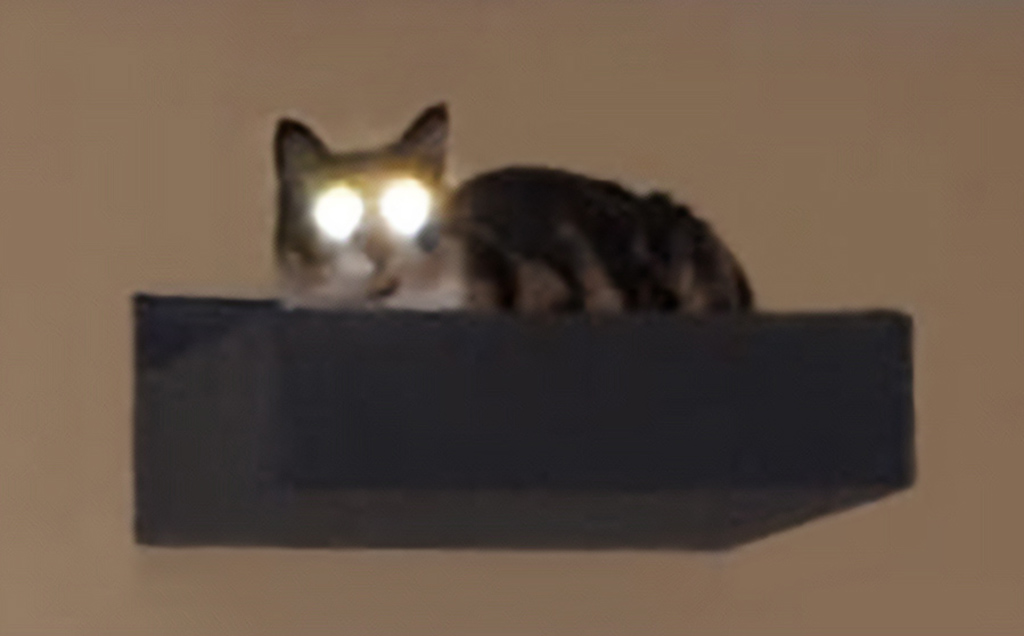
\includegraphics[width=4cm]{figures/taxonomy/cat_eyes.jpg}
} 
} 

%\marginnote{Plato's dialogues are fictitious conversations among philosophers arguing about several topics.}
Plato’s theory of vision (427--347 BC) was very influential. Plato's theory contained both intromission and extramission elements. The following is a fragment of Plato's dialog \booktitle{Timaeus} \cite{Plato360bc}, which provides a description of how the flow produced by the internal fire in the eyes interacts with the external fire to produce sight:

%%``{\em 

\begin{quote}
And of the organs they first contrived the eyes to give light, and the principle according to which
they were inserted was as follows: So much of fire as would not burn,
but gave a gentle light, they formed into a substance akin to the
light of every-day life; and the pure fire which is within us and
related thereto they made to flow through the eyes in a stream smooth
and dense, compressing the whole eye, and especially the centre part,
so that it kept out everything of a coarser nature, and allowed to
pass only this pure element. When the light of day surrounds the stream
of vision, then like falls upon like, and they coalesce, and one body
is formed by natural affinity in the line of vision, wherever the
light that falls from within meets with an external object. And the
whole stream of vision, being similarly affected in virtue of similarity,
diffuses the motions of what it touches or what touches it over the
whole body, until they reach the soul, causing that perception which
we call sight. But when night comes on and the external and kindred
fire departs, then the stream of vision is cut off; for going forth
to an unlike element it is changed and extinguished, being no longer
of one nature with the surrounding atmosphere which is now deprived
of fire: and so the eye no longer sees, and we feel disposed to sleep.
\end{quote}

%%}''
% excerpt from http://classics.mit.edu/Plato/timaeus.1b.txt

Plato considered the sense of vision as being worse than touch because vision could only sense the part that was facing the observer. Therefore, according to Plato, one could not trust the sense of vision. However, Aristotle (384--322 BC), Plato's student, was critical of the extramission theory and pointed out that the stars were too far away for rays from the eyes to reach them (an argument also used by Euclid). Aristotle went further and suggested that only some objects are light sources (e.g., fire) and the other objects reflect the rays that hit the eyes \cite{Aristotle350bc}. He also criticized the belief that the eye had fire inside. Instead, Aristotle defended the idea that the element of perception had to be water as vision needed a transparent element.


Euclid (325 BC), a Greek mathematician, provided the first mathematical theory of vision, giving a mathematical description of how the emitted rays by the eye traveled on {\bf straight lines} and formed a cone that reached the scene. 
\marginnote{Modeling light as traveling along straight lines was a major discovery. This simple model of light sets the foundation upon which image formation, scene geometry, and computer vision rests.
%\begin{figure}
%\centerline
\\[6pt]
\centerline{
%\includegraphics[width=1\linewidth]{figures/taxonomy/eye_w_fire_aina.eps}
\includegraphics[width=4cm]{figures/taxonomy/eye_w_fire_aina.eps}
%}
%\end{figure}
}
}
He listed the following seven axioms of light, extracted from \cite{Burton1945}:
% from http://philomatica.org/wp-content/uploads/2013/01/Optics-of-Euclid.pdf
\begin{quote}
\begin{enumerate}
    \item Let it be assumed that lines draw directly from the eye pass through a space of great extent;
    \item and that the form of the space included within our vision is a cone, with its apex in the eye and its base at the limits of our vision;
    \item and that those things upon which vision falls are seen, and that those things upon which vision does not fall are not seen;
    \item and that those things seen within a larger angle appear larger, and that those seen within a smaller angle appear smaller, and those seen within equal angles appear to be of the same size;
    \item and that things seen within the higher visual range appear higher, while those within the lower range appear lower;
    \item and, similarly, that those seen within the visual range on the right appear on the right, while those within that on the left appear on the left;
    \item but that things seen within several angles appear to be more clear.
\end{enumerate}
\end{quote}

Starting from those axioms, in his paper ``Optics'' \cite{Burton1945}, Euclid describes many different ways to use geometric reasoning to measure the size of objects in the world using the properties of light and vision.  
One example of the application of his theory is shown in \fig{\ref{fig:euclid}}.
The description of the figure in the original text reads as follows: 
%\begin{quote}
``To know how great is a given elevation (AB) when the sun is shining. Let the eye be D, and let GA be a ray of the sun falling upon the end of line AB, and let it be prolonged as far as the eye D. And let DB be the shadow of AB. And let there be a second line, EZ, meeting the ray, but not at all illuminated by it below the end of line at Z. So, into the triangle ABD has been fitted a second triangle, EZD. Thus, as DE is to ZE, so is DB to AB. But the ratio of ED to ZE is known. Moreover, DB is known; so, AB is also known''
%\end{quote} 
\cite{Burton1945}.


\begin{figure}[t]
\centerline{
\includegraphics[width=0.6\linewidth]{figures/taxonomy/euclid.eps}
} 
\caption{Adapted from Euclid (325 BC). The color and text, added here for clarity, is not part of the original figure \cite{Burton1945}. 
%The description of the figure reads \cite{Burton1945}: ``{\bf To know how great is a given elevation (AB) when the sun is shining}. Let the eye be D, and let GA be a ray of the sun falling upon the end of line AB, and let it be prolonged as far as the eye D. And let DB be the shadow of AB. And let there be a second line, EZ, meeting the ray, but not at all illuminated by it below the end of line at Z. So, into the triangle ABD has been fitted a second triangle, EZD. Thus, as DE is to ZE, so is DB to AB. But the ratio of ED to ZE is known. Moreover, DB is known; so, AB is also known."
} 
\label{fig:euclid}
\end{figure}


\marginnote{Euclid's work set the basis of {\bf perspective}, and his discoveries influenced thinkers and artists in the following centuries.}[-0.05in]


Many other Greek philosophers and mathematicians 
contributed to a deeper understanding of light. Hero of Alexandria (10-70), in the work \textbf{Catoptrica}, postulated that light propagated in straight lines and also described an early version of the {\bf law of reflection}: light will follow the shortest path between two points, which means that the angle of incidence is the same as the angle of departure. Ptolemy described how light changed direction (i.e., {\bf refraction}) when changing medium (e.g., from air to water). Few other discoveries about vision between the first and tenth centuries survive.
\marginnote{Credit assignment is unclear. For instance, early versions of the law of reflection are credited to Heron, Ptolemy, Archimedes, Plato, and was potentially known to others before \cite{10.2307/225870}.
% https://www.jstor.org/stable/225870
}



In the late tenth century Hasan Ibn al-Haytham's work transformed the initial Greek theories into a true scientific discipline, inspiring many of the works that followed, even through Johannes Kepler.  Ibn al-Haytham (965--1040 AD), known as Alhacen in the Latin world, published the \booktitle{Book of Optics} \cite{2001alhacen} between the years 1028 and 1038. This book is considered by many the beginning of the scientific method. In his Book of Optics, Ibn al-Haytham describes how light rays bounce of objects in all directions and that the rays only become visible when they reach the eye perpendicularly. He described the pinhole camera and invented the {\bf camera obscura}. 
\index{Camera obscura}


\begin{figure}[t]
\centerline{
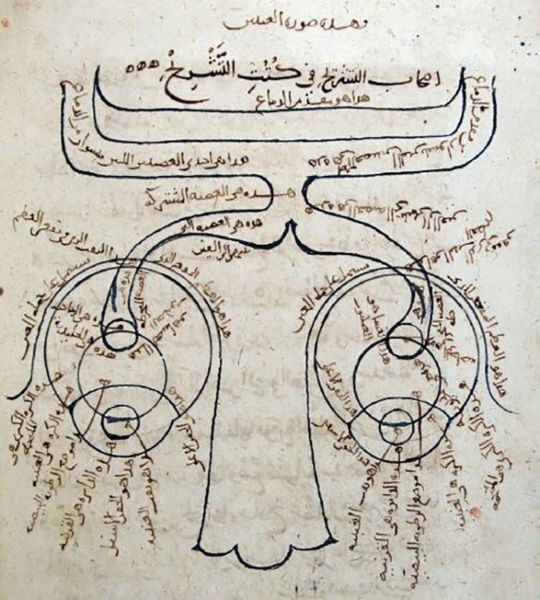
\includegraphics[width=0.5\linewidth]{figures/taxonomy/Alhazen1652.png}
% https://www.discovermagazine.com/mind/visions-of-the-brain-ancient-and-modern
% http://glps2.org/wiki/index.php?title=File:Alhazendiagramnerves.gif
% https://www.aspetar.com/journal/viewarticle.aspx?id=293#.Yo42TGDMJO5
} 
\caption{Alhacen's diagram of the eyes and the optic nerve (\booktitle{Book of Optics}), drawn around the year 1027. It is one of the first drawings of the visual system. {\em Source}: MS Fatih 3212, vol. 1, fol. 81b, Süleimaniye Mosque Library, Istanbul.} 
\label{fig:Alhacen}
\end{figure}


Ibn al-Haytham rejected the extramission theory. He argued that sight could be explained by the light rays emitted by objects and that it was not necessary to assume that the eye emitted rays. Ibn al-Haytham's work built upon the work of Ptolemy, Euclid, Galen, and Aristotle, although little is known about the exact sources of inspiration as manuscripts at that time did not include citations to previous work and it was rare when other scientists were cited by name. Ptolemy believed that distance between the eye and an object could be measured by feeling the length of a ray of light (thus requiring a single eye), while Ibn al-Haytham showed experimentally that both eyes were needed to perceive depth \cite{2001alhacen}.



Kepler (1604 AD), building on Alhacen's work, provided the first complete description of how images are formed in the retina in \booktitle{Astronomiae Pars Optica} 
%Ad Vitellionem paralipomena 
\cite{Martens2001-MAROPT-2}. Kepler understood {\bf lenses} and how the eye projected a reverse picture into the retina. Kepler understood the role of the crystalline lens as the focusing element of images in the eye, in contrast with previous theories that believed that the crystalline lens was the sensitive element selecting only the perpendicular rays that reached the eye.  



\subsection{Helmholtz: Perception as Inference}


Hermann von Helmholtz (1821--1894) was a German scientist and philosopher. While he wanted to study physics, he trained as a physician at the urging of his father \cite{Shapin2019}, then went on to make important contributions in philosophy, physics, audition, color theory, and visual perception.


With Thomas Young, he codeveloped the theory of {\bf trichromacy}, 
\index{Trichromacy}
that the eye has three classes of receptors, each sensitive to different wavelengths of light.  \marginnote{
\centerline{

\includegraphics[width=3cm]{figures/taxonomy/trichromacy_helmholtz.eps}
}
}

He measured the speed of transmission of nerves (24.6--38.4 m/s \cite{wikiHelmholtz2021}, previously thought to be unmeasurably fast \cite{Shapin2019}).  He also developed the ophthalmascope, shown in \fig{\ref{fig:helmholtz}}, an instrument to observe the retina of the human eye. The key of the ophthalmascope was to see the need for colinear viewing and illumination directions. \Fig{\ref{fig:helmholtz}}{a} shows a schematic illustration of Helmholtz's opthalmoscope, viewed from above.  The glass plates along the diagonal, labeled $a$ in the figure, allow for viewing the eye under study by the opthalmologist while reflecting illumination from a light source into the eye. \Fig{\ref{fig:helmholtz}}{b} shows a drawing by Helmholtz of an image from the ophthalmoscope, showing blood vessels (in background) and branches of the retinal artery and vein over the optic nerve (center). 


\begin{figure}[t]
\centerline{
\sublabel{a}{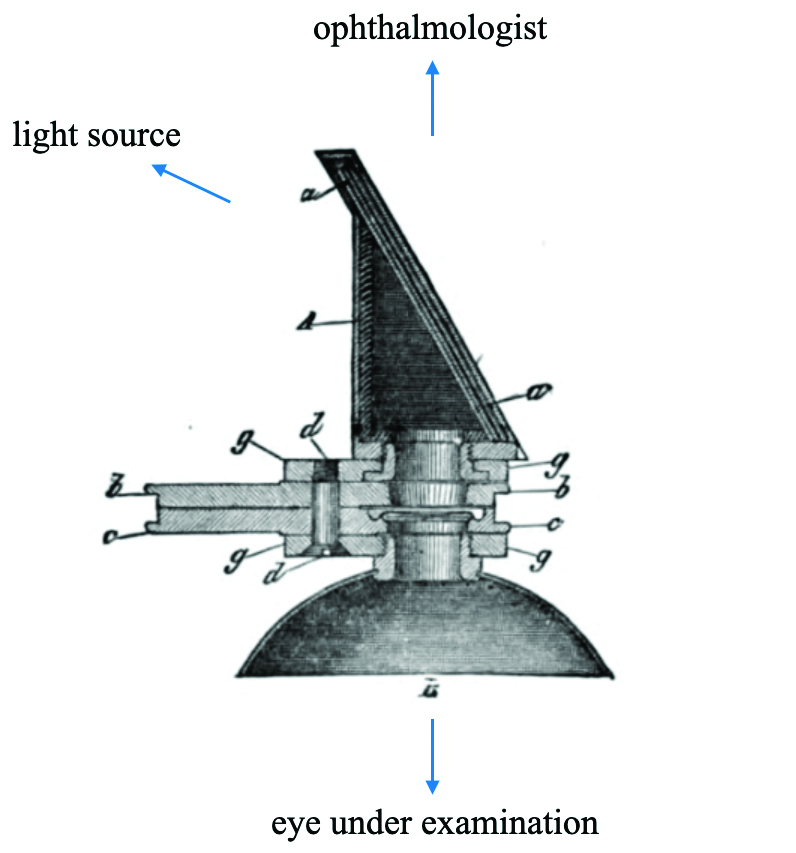
\includegraphics[width=0.45\linewidth]{figures/taxonomy/helmholtzOpth1Labeled.jpg}}
\sublabel{b}{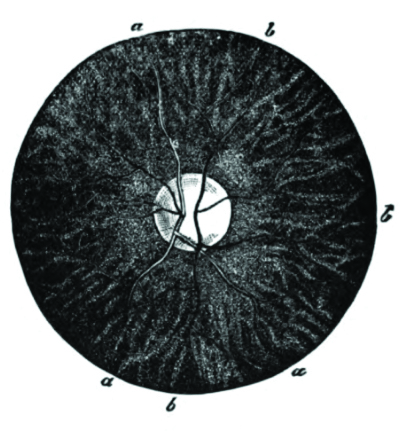
\includegraphics[width=0.44\linewidth]{figures/taxonomy/helmholtzOpth3.jpg}}
} 
\caption{Hermann von Helmholtz invented the ophthalmoscope at age 29.  
%The key was to see the need for colinear viewing and illumination directions. (a) Schematic illustration of Helmholtz's opthalmoscope, viewed from above.  The glass plates along the diagonal, labeled $a$ in the figure, allow for viewing the eye under study by the opthalmologist while reflecting illumination from a light source into the eye. (b) Drawing by Helmholtz of an image from the ophthalmoscope, showing blood vessels (in background) and branches of the retinal artery and vein over the optic nerve (center).  
Images from \cite{Helmholtz1925}.}
\label{fig:helmholtz}
\end{figure}


Helmholtz was also an important theorist in visual perception.  He wrote \cite{Helmholtz62}, 
%``
\begin{quote}
The general rule determining the ideas of vision that are formed whenever an impression is made on the eye, is that {\em such objects are always imagined as being present in the field of vision as would have to be there in order to produce the same impression on the nervous mechanism, the eyes being used under ordinary normal conditions}.
%''
\end{quote}
%(Emphasis in the original) \cite{Helmholtz62}.

Thus, the mind makes perceptions out of sensations \cite{Shapin2019}, finding representations of the object most likely to explain the sensory input \cite{Wandell95}.  This viewpoint relates to {\bf Bayesian methods} for computer vision inference.

In his introduction, ``Concerning the Perceptions in General,'' he continued \cite{Helmholtz62}:
\begin{quote}
%``
Still, it may be permissible to speak of the psychic acts of ordinary perception as {\em unconscious conclusions}, thereby making a distinction of some sort between them and the common so-called conscious conclusions.
\end{quote}
%''
He added that when an astronomer computes the position of stars in space, based on observations, this is a conscious conclusion. When you press on the eye and see light, that is an unconscious conclusion about what is in the world, given the responses of your eye. This unconscious inference is the topic of computer vision.


Helmholtz emphasized the active role of the viewer in perception \cite{Helmholtz62},
\begin{quote}
If the objects had simply been passed in review before our eyes by some foreign force without our being able to do anything about them, probably we should never have found our way about amid such an optical phantasmagoria ... But when we notice that we can get various images of a table in front of us simply by changing our position; and that we can sometimes have one view and sometimes another, just as we like at any time ... Thus by our movements we find out that it is the stationary form of the table in space which is the cause of the changing image in our eyes.
\end{quote}
This foreshadows some unsupervised learning methods common in computer vision today.


\subsection{Gestalt Psychology and Perceptual Organization}
% https://www.ncbi.nlm.nih.gov/pmc/articles/PMC3482144/
% https://www.sciencedirect.com/science/article/pii/S0042698900000869?via%3Dihub


Gestalt psychology 
\index{Gestalt psychology}
started around 1912, with the publication of “Experimental Studies of the Perception of Movement” by Max Wertheimer \cite{wertheimer1912experimentelle}. In this paper Wertheimer introduced the {\bf phi phenomenon}, a visual illusion that consists in presenting two images with a vertical bar at different locations in rapid succession giving the impression that there is continuous motion between them \cite{steinman2000phi}. 
\marginnote{
\centerline{Frame 1 ~~~~~~~~~~~~~~~~~~~~~~~~~~~~~~~~~~~~~~~~~~~~~Frame 2}
~\\[-4pt]
\centerline{
\includegraphics[width=.35\linewidth]{figures/taxonomy/phi_phenomenon_1.eps}
~~
\includegraphics[width=.35\linewidth]{figures/taxonomy/phi_phenomenon_2.eps}
}
}
Wertheimer, together with Kurt Koffka and Wolfgang Köhler, postulated that perceived motion was a new phenomenon that is not present in the individual stimuli (the two flashing frames) and that what we perceive is the whole event as a single unit (continuous motion). Gestalt psychology extended this interpretation to explain many other visual phenomena and emerged as a reaction of the existing trend that said that for psychology to be a science it had to decompose stimuli into its constituent elements. Gestalt theory argued that perception is about wholes more than it is about parts.



Wertheimer introduced the problem of {\bf perceptual organization}. 
\index{Perceptual organization}
Perceptual organization studies how our visual system organizes individual visual features (i.e., colors, lines, ...) into coherent objects and wholes. Wertheimer proposed a set of rules
used by the visual system to organize elements on a simple display. He showed sets of dots and lines disposed in different arrangements, as shown in \fig{\ref{fig:gestalt}}, to find out when those elements were grouped together into larger elements.  


\begin{figure}[t]
\centerline{
\includegraphics[width=1\linewidth]{figures/taxonomy/gestalt.eps}
} 
\caption{Gestalt grouping rules for perceptual organization. Most of the examples are recreated from \cite{Palmer1999}. The closure pattern is from Koffka \cite{Koffka1935}, who modified it from Kohler.} 
\label{fig:gestalt}
\end{figure}

Gestalt psychologists called {\bf grouping laws} 
\index{Gestalt psychology!Grouping laws}
the visual cues they uncovered. However, they are not strictly laws and not all grouping cues are equally strong. Some of the most important laws are as follows:
\begin{itemize}
    \item Law of {\bf proximity}: Items that are nearby are more likely to group together. From \fig{\ref{fig:gestalt}}, we can see that groupings a-b, c-d, e-f, and g-h are stronger than b-c, d-e, and f-g. With some effort one can group the items according to the second arrangement, but it is hard to sustain that grouping perceptually. The law of proximity is affected by the similarity of the items. 
    \item Law of {\bf similarity}: Elements that have similar features (color, size, orientation) also group together, even when they are all equally distant. 
    \item Law of {\bf closure}: We are very familiar with the fact that when a line forms a closed figure, we do not simply see a line, we see a shape. The example shown in \fig{\ref{fig:gestalt}} shows how closure wins over proximity. The vertical lines are closer for the grouping a-b. However, we group them as b-c, d-e, and f-g. 
\item Law of {\bf good continuation}: Edges are likely to be smooth. Lines that follow each other pointing in the same direction are likely to be grouped together. For instance, an X-shape is perceived as two lines that cross each other instead of perceiving it as a V-shape on top of an inverted V.
\marginnote{Law of good continuation. The following shape: 
\\[6pt]
\centerline{
\includegraphics[width=.15\linewidth]{figures/taxonomy/grounding_gc_1.eps}}
has two possible groupings:
\\[6pt]
\centerline{
\includegraphics[width=.35\linewidth]{figures/taxonomy/grounding_gc_2.eps}}
The law of good continuation says that the one on the left is 
the one an observer perceives (although we just see an X and not two lines crossing each other...)
}[-.2in]

    \item Laws of {\bf parallelism}, and {\bf symmetry}: There are many other grouping cues with different strengths that induce clustering between visual elements. 
    \item {\bf Common fate}: Motion is a very important grouping cue. When two elements have a common motion (accelerations, direction, rate of change) they tend to group together.
    %\item Law of prägnanz or simplicity
    \item {\bf Past experience}: Items grouped in the past are more likely to be perceived as a group in the future. 
    %Palmer \cite{Palmer1999} highlighted the importance of this grouping introduced by Wertheimer.
\end{itemize}

 In complex displays, one will expect that multiple of these grouping cues will be present. Gestalt theory not did quantitatively address how grouping cues will balance each other when they were in conflict. Stephen Palmer \cite{Palmer94} measured the strength of these grouping cues and introduced new ones. 

Gestalists also studied the problem of {\bf lightness perception}. 
\index{Lightness perception}
\marginnote{
{\bf Lightness} is a perceptual quantity that is influenced by both the perceived reflectance and the perceived illumination of a surface \cite{Adelson99}. 
%Ted Adelson \cite{Adelson99} defines {lightness} as "the perceived reflectance of a surface. It represents the visual system’s attempt to extract reflectance based on the luminances in the scene". And Reflectance "is the proportion of incident light that is reflected from a surface."
}
For a wonderful book on lightness perception, we refer the reader to \cite{gilchrist2006}, and the work of Edward Adelson \cite{Adelson99}. Adelson defines lightness as ``the visual system’s attempt to extract reflectance based on the luminances in the scene.''

Gestalt psychologists said that the perception of lightness on an image patch is a function of the context. One has to take into account the grouping laws (perceptual organization) in order to explain the perceived lightness on a display. Koffka \cite{Koffka1935} introduced the {\bf Koffka ring}, a beautiful illusion to illustrate the power of perceptual grouping to explain lightness perception (\fig{\ref{fig:koffka_ring}}). 
\marginnote{Kurt Koffka, born in Berlin in 1886, published his \booktitle{Principles of Gestalt Psychology} in 1935, after moving to the USA in 1924.}

\begin{figure}[t]
\centerline{
\includegraphics[width=1\linewidth]{figures/taxonomy/koffka_ring.eps}
} 
\caption{(a) A ring of uniform gray. (b) Koffka ring and (c) a variant introduced by Adelson \cite{Adelson99}.  In all the examples, the two sides of the ring are identical.} 
\label{fig:koffka_ring}
\end{figure}

In each display, the two sides of the ring have the same gray level. Depending on the spatial configuration of the two sides, their lightnesses appear very different. In \fig{\ref{fig:koffka_ring}}{a} the ring appears as solid gray. In \fig{\ref{fig:koffka_ring}}{b} splitting the figure into two halves by an interleaving white space makes the two sides of the ring look different. \Fig{\ref{fig:koffka_ring}}{c} shows a variant of the Koffka ring proposed by Adelson \cite{Adelson99} where the grouping cues create a stronger effect. One can conclude from this experiment that lightness perception is not a local process and that it involves considering the context and the principles of grouping.



%Koffka, born in Berlin in 1886, moved to USA in 1924. In 1935, Koffka published his Principles of Gestalt Psychology.


Another striking proof of the importance of perceptual organization is the visual phenomenon of {\bf amodal completion}. 
\index{Perceptual organization!Amodal completion}
As discussed in the introduction, in \fig{\ref{fig:measuringScene}}{a} we see a red square on top of a blue square. Even though the blue square is occluded by the red square, we see it as a square. The green geometric figure is identical to the blue one but the gap breaks the illusion of occlusion and we do not perceive it as a square anymore. This phenomenon of perceiving a whole object when only a part is visible is called {\bf amodal completion}. The word {\em amodal} means that we have perception without using any direct perceptual modality. 

Amodal completion is something we do all the time when we explore a scene. Most of the objects that we see are partially occluded and we use amodal completion to extend the object behind the occlusion. 

{\bf Modal completion} 
\index{Perceptual organization!Modal completion}
is a related visual phenomenon that happens when we see an induced object appear in front of others. \Fig{\ref{fig:kanizsa}} shows several examples of modal and amodal completion. A beautiful visual illusion that illustrates modal completion is the {\bf Kanizsa triangle}, shown in \fig{\ref{fig:kanizsa}}{d}. In this case, we see a triangle that is not really there. 


\begin{figure}
\centerline{
\includegraphics[width=1\linewidth]{figures/taxonomy/kanizsa.eps}
} 
\caption{Amodal and modal completion. (a) is this 13 or an occluded B? (b) By adding boundaries to the occluder, the letter B becomes clearer. (c) How many squares are there? Behind the occluder are there two squares or just one rectangle? (d) Kanizsa triangle. Illusory contours appear at the triangle sides.} 
\label{fig:kanizsa}
\end{figure}

The Kanizsa triangle shows both amodal and modal completion. The circles are seen by amodal completion and the triangle appears as modal completion. Modal completion produces {\bf illusory contours} to appear in the image. Some observers report that the triangle on top is brighter than the surrounding background and that illusory contours appear at the triangle sides.
\index{Perceptual organization!Illusory contours}

\marginnote{Gaetano Kanizsa \cite{kanizsa79} studied how perceptual organization could be used to see what is not there.} 

% Specially remarkable is the Kanizsa triangle, Figure.~\ref{fig:kanizsa}.d. The circles are amodally completed, the invisible triangle is modally completed. 


%Organization in Vision: Essays on Gestalt Perception, Praeger Publishers, 1979

Perceptual organization remains an intriguing and rich area of research with many visual mechanisms still poorly understood. The list of principles of perceptual organization discovered by the gestalt theory have impacted a lot of modern research in computer vision, in particular in the domain of {\bf image segmentation} \cite{Malik90}.


\subsection{Gibson's Ecological Approach to Visual Perception}

While previous theories of perception considered that the simplest scenario to study vision was assuming a static camera taking a snapshot in a controlled lab setting, James J. Gibson postulated that, to understand vision, one should take an {\bf ecological approach to visual perception} \cite{Gibson1979}. The study of the eye should be done in the context of the body that supports it and the world it lives in.

Experimental science based in simple visual stimuli allowed for measuring quantities, reporting results, and reproducing findings, but the simple stimuli were very limiting. Dealing with real-world stimuli is messy, and no one had good theories on how to use them experimentally. Gibson argued that, to understand perception, the experimental lab should be like real life. Many of the displays used by gestalt psychologists were too simple and unlikely to occur in the real world. They provide useful knowledge, but fall short of unraveling the true nature of the visual system. 

The environment should be studied by means of ecological properties, and not by using physical laws. That is, by understanding what quantities and processes of the environment are relevant for the observer. An ecological description of the environment describes it in terms of medium (air or water), substances (rocks, metal, wood, etc.), and surfaces (which separate medium from substances), together with the notions of change and persistence. 
Gibson considers those concepts more relevant to the study of perception than the notions of space, matter, and time, which have their origin in classical physics but have little relevance for the observer. The dominant role of the observer in Gibson's theory is illustrated in how the environment is understood: water is substance for terrestrial animals, and it is the medium for aquatic animals. 
The {\bf ground plane} 
is the most important surface for terrestrial animals, it is the center of their perception and behavior. The ground provides the support for action and a reference for perception. Other notions of ecological importance are the concepts of {\em layout}, {\em place}, and {\em enclosure}. 
\marginnote{Drawing by Gibson showing how few lines induce a strong 3D percept of a ground plane.
\\[6pt]
\centerline{
\includegraphics[width=.3\linewidth]{figures/taxonomy/gibson_cover_the_perception_of_visual_world.eps}
} 
} 


Gibson also made a distinction between the light studied by optical physics and the one that is relevant for perception, which he called {\bf ecological optics}. 
\index{Ecological optics}
According to Gibson, physicists are interested in studying light in simplified settings such as the light emitted by point sources that send rays into an infinite space, or that interact with surfaces or lenses once. Ecological optics instead studies the light that converges into the observer, which is the result of countless interactions with all the surfaces in a messy environment. The {\bf ambient optic array} is the set of light rays that converge into a point of observation. And this point of observation can be occupied by an observer who will move around the world. This moving ambient optic array will contain information about the environment and also about the observer themself (\fig{\ref{fig:gibson_bird}}). 


\begin{figure}[t]
\centerline{
\includegraphics[width=0.7\linewidth]{figures/taxonomy/gibson_bird.eps}
} 
\caption{The flow pattern in the optic array of a bird flying over the earth provides information about the environment and also about the bird. Figure recreated from \cite{Gibson1966}.} 
\label{fig:gibson_bird}
\end{figure}

Another key concept in Gibson's theory is the notion of {\bf affordance} \index{Affordance}
introduced by Gibson in 1966 \cite{Gibson1966}. A {\em path} affords locomotion from one point to another, an {\em obstacle} affords collision, and a {\em stairway} affords both descent and ascent. 
%The Senses Considered as Perceptual Systems, 1966
An {\em object} is a substance enclosed by a surface. The affordance of an object is generally a direct consequence of its properties: a hollow object can contain substances, a detached object affords carrying, an object with a sharp edge affords cutting, and so on. Animate objects are controlled by internal forces, and they afford social interaction. 


Gibson's theory of visual perception postulates that the ambient optic array is very rich and contains all the information needed to perceive the environment.  {\bf Direct perception} is the process of {\bf information pickup} directly from the ambient array. This is in contrast with other theories of visual perception that assume that the input stimuli
\marginnote{Gibson did not like the term {\bf stimuli} because it implied that the environment stimulates the observer. For Gibson, it is important to stress that the observer is only picking up information.}[-.3in] 
is very impoverished and that perception is {\bf indirect} as it has to be complemented by additional processes.
The indirect theory of perception is the most common one. However, the important message to learn here is that, when building a perceptual system, the richer the input is, one might hope that the solution to the perception problem will be simpler. 
% For a discussion on direct vs. indirect: https://media.pluto.psy.uconn.edu/MC.pdf

% Modern studies on natural scene understanding and the statistical properties of natural images have been greatly influenced by Gibson's ideas.


\subsection{The Neural Mechanisms of Visual Perception}

Neuroscience has greatly contributed to our understanding of how vision works and has inspired a large number of computer vision approaches: red-green-blue (RGB) encoding of images, filter based image representations, neural networks, and attention modulation. Studies on the neural mechanisms of visual perception had a lasting impact. In this section will only review some of the many discoveries made over many centuries trying to explain how the brain works. One premise in the computational neuroscience community is that one can understand how vision works by reverse engineering how the brain solves the task.

For a long time it was known that the brain was the center of reason, but the mechanisms and anatomy of the brain were not well understood. In fact, researchers believed that the brain was not composed of individualized cells as the rest of the body. 
It was in 1890 that Santiago Ram\'{o}n y Cajal, using Golgi's stain, 
\marginnote{Santiago Ram\'{o}n y Cajal was born in 1852 in Navarra, Spain.}
isolated individual neurons and proved that the brain is composed by {\bf networks of interconnected cells} as shown in his work on the anatomy of the retina \cite{cajal1893retine}. This was the first time that networks were observed. Ram\'{o}n y Cajal then mapped most of the brain and his drawings are still a reference. Both Santiago Ram\'{o}n y Cajal and Camillo Golgi received the Nobel prize in 1906 \cite{Glickstein2006}. 


\begin{figure}
\centerline{
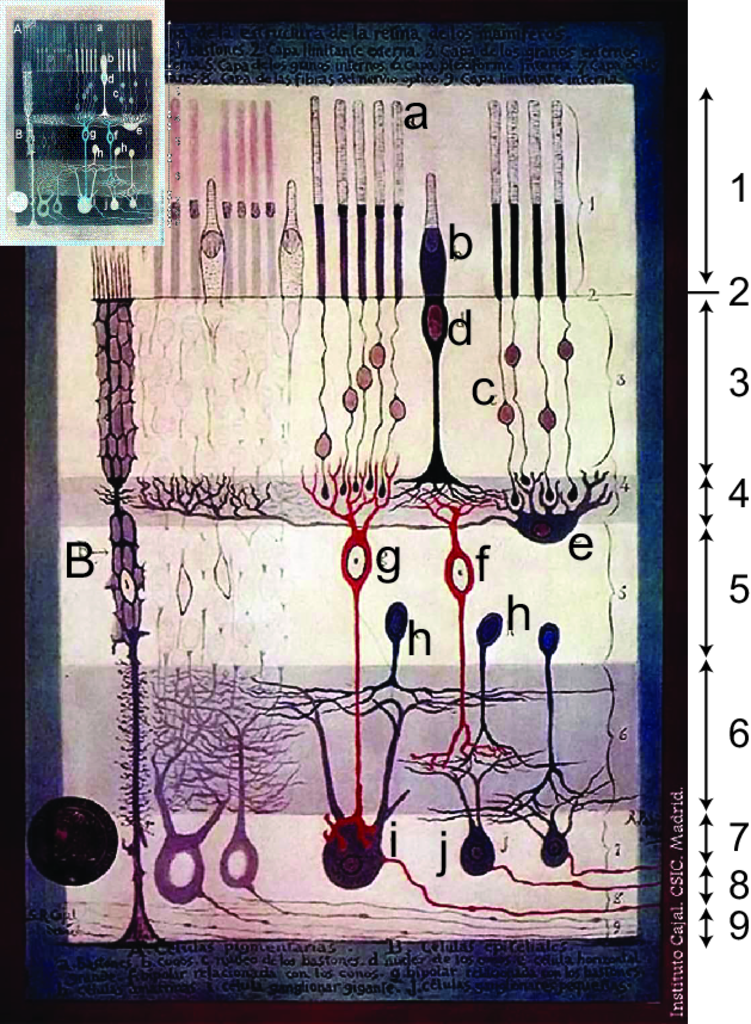
\includegraphics[width=.6\linewidth]{figures/taxonomy/cajal.eps}
} 
\caption{Drawing of the retina by Santiago Ram\'{o}n y Cajal. In this drawing photoreceptors are in the top and light comes from the bottom: 
%(indeed, light needs to traverse all the layers of the retina before reaching the light sensitive layer). 
 1. Rod and cone layer. 2. External limiting membrane. 3. Outer granular layer. 4. Outer plexiform layer. 5. Inner granular layer. 6. Inner plexiform layer. 7. Ganglion cell layer. 8. Optic nerve fibre layer. 9. Internal limiting membrane. A. Pigmented cells. B. Epithelial cells. a. Rods. b. Cones. c. Rod nucleus. d. Cone nucleus. e. Large horizontal cell f. Cone-associated bipolar cell. g. Rod-associated bipolar cell. h. Amacrine cells. i. Giant ganglion cell. j. Small ganglion cells.  
%modified from \url{https://commons.wikimedia.org/wiki/File:Cajal_Retina.jpg}, originally 
{\em Source}: ``Structure of the Mammalian Retina'' c.1900 By Santiago Ramon y Cajal.} 
\label{fig:cajal}
\end{figure}


The drawing of the retina (\fig{\ref{fig:cajal}}) shows the first layers of neurons that process the visual input. The retina is an amazing piece of the brain that transforms light into impulses. Light is first transformed into electric signal by the photoreceptors 
\index{Photoreceptors}
(rods and cones) and is then processed by a few layers formed by several types of neurons (amacrine, bipolar, and ganglion cells). Finally, ganglion cells transmit the output of the retina through the optic nerve to the rest of the brain. The studies of Ram\'{o}n y Cajal revealed the circuitry of many parts of the brain but told us little about their functional behavior or how the circuits were processing information. 

The {\bf retina} 
\index{Retina}
was one of the first visual structures that was studied from a functional perspective. Haldan Keffer Hartline \cite{Hartline1938}, in 1938, using an innovative method to record the response of single optic nerve fibers (which corresponds to the axons of ganglion cells),  
studied retinal ganglion cells and popularized the concept of {\bf receptive field}, previously introduced by Charles Scott Sherrington \cite{Sherrington1906} in 1906 when studying the tactile domain. 

\marginnote{A review of how the concept of {\bf receptive field} evolved can be found in \cite{Spillmann2014ReceptiveFO}.}

The receptive field of a  neuron corresponds to the region of the input stimulus space (the retina in the case of a visual neuron) that has to be stimulated in order to produce a response in the neuron. Most neurons in the visual processing stream are activated only when light shines on a precise portion of the retina.

\marginnote{Only stimulation within the {\bf receptive field} (RF) of a neuron produces a response.
\\[6pt]
\centerline{
\includegraphics[width=.4\linewidth]{figures/taxonomy/receptive_field.eps}
}
}

Steven Kuffler (1953) studied the organization of the retina and showed that ganglion cells have concentric receptive fields with a circular {\bf center-surround organization} \cite{Kuffler1953}. 
\index{Receptive field}
He did this by shining a small spot of light on different parts of the retina and recording the response of a ganglion cell as he changed the location of the spot of light. First Hartline, and then Kuffler, showed that there were two types of ganglion cells; a first group of cells, called {\bf on-center}, would get activated when the spot of light was inside a small region in the middle of the receptive field and would get deactivated (firing bellow their average rate) when the spot light was projected inside a ring around the center. 
A second group had the opposite behavior, called {\bf off-center}. These results are fascinating because they reveal that the retina seems to be performing some sort of contrast enhancing operation (as we will discuss in other chapters) and their work motivated a large number of studies in {\bf computational neuroscience} and {\bf neuromorphic engineering} \cite{Mead89} that tried to reproduce the operations made in the retina. Haldan Keffer Hartline received the Nobel Prize in 1967 for his discoveries on how the eye processes visual information. 


The axons of ganglion cells from both eyes projects to another structure called the {\bf lateral geniculate nucleus} (LGN). The LGN is composed of six layers of neurons and its output goes to the visual cortex and other visual areas. This structure receives inputs from both eyes but the signals are not mixed and the neurons in this area remain monocular. LGN neurons have concentric (center-surround) receptive fields. The role of the LGN is not completely understood but it may be involved in temporal decorrelation, attention modulation and saccadic suppression. Interestingly, only 5 percent of the input connections come from the retina while 95 percent of the LGN inputs are {\bf feedback connections} from the primary visual cortex and other areas. 


Concentric receptive fields are very common in the early layers of visual processing, but things become more interesting when studying cells in the {\bf visual cortex}. One challenge was that the techniques used to record the responses of cells in the optic nerve could not be applied to record the activity of cells in the cortex. \Fig{\ref{fig:receptivefields}} shows some of the receptive fields found in the LGN. When a cell with an {\bf ON-center Receptive Field (RF)} is illuminated with a small spot of light projected on the inner part of the RF, the firing rate increases, as shown in \fig{\ref{fig:receptivefields}}{a}. The gray rectangle under the graph represents the duration of the stimulation. When the outer part of the RF is stimulated there is an inhibition of the cells response. \Fig{\ref{fig:receptivefields}}{a} shows an {\bf OFF-center RF}.


\begin{figure}[t]
\centerline{
\includegraphics[width=1\linewidth]{figures/taxonomy/receptive_fields.eps}
} 
\caption{Receptive fields (RF) for retinal ganglion cells and oriented receptive fields from the primary visual system. (a) ON-center RF. (b) OFF-center RF. (c-d) Two types of oriented simple cell. (e) Sketch of the response of the cell from (c) to an oriented bar with different orientations in the center of its RF. The gray bar corresponds to the moment the bar is visible.} 
\label{fig:receptivefields}
\end{figure}

% https://www.cns.nyu.edu/~david/courses/perception/lecturenotes/ganglion/ganglion.html
Between 1955 and 1958, David H. Hubel invented a microelectrode that allowed him to record the activity of individual cells in the cortex. He then went to work with Torsten N. Wiesel in Kuffler's lab. They used Hubel's technique to record the response of cells in the visual cortex of cats; this work resulted in them receiving the Nobel prize in 1981.


% https://www.ncbi.nlm.nih.gov/pmc/articles/PMC1363130/pdf/jphysiol01298-0128.pdf

In 1959, Hubel and Wiesel published the study that marked the beginning in understanding how visual information is processed in the brain \cite{HubelWiesel59}. They studied 45 neurons for a period of two to nine hours from the striate cortex on an anesthetized cat. They exposed each neuron to a diverse set of visual stimuli containing spots of various sizes and locations, and {\bf oriented bars}. For most of the neurons they could locate a region of the retina that produced a firing of the neuron when stimulated with light. However, not all types of visual stimuli were effective in driving neurons at the cortical level. %In general, large circular spots of light were ineffective. 
% Original text: In most units it was possible to find a restricted area in the retina from which firing could be influenced by light. This area was called the receptive field of the cortical unit, applying the concept introduced by Hartline (1938) for retinal ganglion cells. 

Hubel and Wiesel discovered that some neurons in the visual cortex were best stimulated by an oriented bar at an specific orientation when it appeared at the center of the neuron's receptive field. They found different types of cells in the primary visual cortex, some that were similar to those found in the retina and LGN (center-surround), others selective to oriented bars, and more complex ones.
They classified each cell according to its attributes: spatial selectivity, orientation preference, eye preference (left or right), and the type (simple, complex, or hypercomplex).

\Fig{\ref{fig:receptivefields}}{c} shows an {\bf oriented simple cell}, while \fig{\ref{fig:receptivefields}}{d} shows another type of simple oriented cell found in the visual cortex. An oriented cell shows increased firing rate when stimulated with an oriented bar in the positive region of the RF with the preferred orientation.
\index{Visual cortex}

% https://www.cns.nyu.edu/~david/courses/perception/lecturenotes/V1/lgn-V1.html
\Fig{\ref{fig:visual_pathways}}
shows a schematic of the visual pathways from the retina up to the primary visual cortex.The first visual area in the visual cortex is called {\bf V1}. It is a sheet of neurons is arranged along several layers as shown in \fig{\ref{fig:visual_pathways}}. %Neurons in V1 are organized along {\bf columns} creating arrangements with nearby neurons having similar preferred orientations, with a smooth transition from one part of the visual cortex to another and with alternance in eye preference.  
Hubel and Wiesel found that neurons in V1 are organized along {\bf columns}. When probing with an electrode, as the electrode went from the surface to the bottom of V1, all the cells found were selective to the same orientation. When moving the electrode along one horizontal direction, they found that the preferred orientation changed smoothly (orientation columns), and when moving the electrode along the perpendicular horizontal direction, the cells changed the eye preference, alternating between the two eyes with some binocular cells between them (ocular dominance columns). A section of around 1 $\times$ 3 mm (called a {\bf hypercolumn}) 
\index{Hypercolumn}
covers all orientations and both eyes for a small portion of the visual field.  

Margaret Livingston, in collaboration with David Hubel, discovered color sensitive neurons \cite{Livingstone1984AnatomyAP} organized in blobs surrounded by orientation-sensitive neurons in the visual cortex.  
%% The schematic is just a sketch that should not be taken too seriously but it reflects the actual structural organization of the vision system. In biology, hardware and algorithm are tied together constraining each other.   ****** I don't feel this sentence adds anything--Bill.


\begin{figure}[t]
\centerline{
\includegraphics[width=.7\linewidth]{figures/taxonomy/visual_pathways_aina.eps}
} 
\caption{Visual pathways. The retina projects the axons of the ganglion cells into the lateral geniculate nucleus (LGN). In each hemisphere, the LGN gets inputs from both eyes (the LGN on the right gets the right side of each retina, which corresponds to the left side of the visual field). The output of the LGN is divided into three channels; the parvocellular, magnocellural, and koniocellular (not shown). Those channels project into the primary visual cortex following a very regular architecture organized along hypercolumns. The koniocellular pathway projects into the color blobs in the upper layer of the visual cortex. Figure modified from \cite{kandel:neural}.} 
\label{fig:visual_pathways}
\end{figure}

\marginnote{Compare the drawing from \fig{\ref{fig:visual_pathways}} with the one made a thousand years earlier by Ibn al-Haytham, shown in \fig{\ref{fig:Alhacen}}.}


Cells in the visual cortex project their outputs to a diverse set of other visual areas following two main streams (the ventral stream and the dorsal stream) and project into specialized areas performing motion processing (area MT), face processing (fusiform face area [FFA]; see\cite{Kanwisher1997TheFF}), and object recognition (IT).

As a result of all those discoveries in neuroscience, a large community of interdisciplinary researchers developed models trying to explain the function of visual neurons. Many of the neurons in the early layer of visual processing (retina, LGN, and visual cortex) can be approximated by linear filters with rectifying nonlinearities and contrast control mechanisms, which are the basis of many computer vision algorithms as we will see throughout this book. 


%``At the cortical level a circular spot was often ineffective; for best driving of each unit it was necessary to find a spot with a particular form and orientation."




%Face area

%Place cells

%Motion area

%Computational neuroscience
%A number of studies tried to 
%Color coding,
%Attick for the ganglion cells, retinal response
%Bruno, David: Cortex


\subsection{Marr's Computational Theory of Vision}


David’s Marr influential book \booktitle{Vision} was published posthumously in 1982 \cite{Marr82}. 
%David Marr started as a
Marr’s philosophy was influenced by advances in computer vision, and studies in cognitive psychology and neurophysiology. Studies in psychology at the time suggested that visual information was processed by independent modules of perception, each one devoted to a specific task (stereo vision, motion perception, color processing), and that visual images were analyzed by independent spatial-frequency-tuned channels. Progress in neurophysiological experiments using single cell recordings showed a strong connection between perception and neural activity. In the 1970’s, computer vision was already a well-established field. Some of the advances that inspired Marr's philosophy were the work by David L. Waltz \cite{Waltz1972GeneratingSD} on the interpretation of block worlds, Edwin H. Land and John J. McCann’s Retinex theory about color perception \cite{Land1971}, and Berthold Horn’s theory of shape from shading \cite{Horn1977}, among many other works.

David Marr, together with Tomaso Poggio and others, postulated that it was important to separate the analysis of the task being solved from the particular mechanism used to solve it \cite{Marr82}. Marr said that the vision problem should be understood at different levels, and that what was missing in previous theories of vision was to understand vision as an {\bf information-processing task}. Marr proposed that an information-processing device should be described at three levels:

\begin{itemize}
\item {\bf Computational theory}. This level of description should answer the following questions: what is the task to be perform and why should it be carried out? In the case of vision, the task is to derive properties of the world from images. This level of description should specify what the mapping is between the input and output, and why this mapping is appropriate for the task that the device needs to solve. This level does not specify how that mapping should be constructed or which algorithm will implement it.  
\item {\bf Representation}. We should define which representation will be used for the input and output. The representation is a system of making explicit certain types of information present on a signal. For instance, an image could be represented by the sequence of values that encode the color of each pixel, but it could be also represented using a Fourier decomposition. The choice of representation will make explicit certain type of information while hiding other information, which will become harder to access. The algorithm used to implement the mapping between input and output will be strongly dependent on the representation used. The importance of the choice of representation is very present in today’s computer vision community. Examples such as using position encoding to represent location illustrate the dramatic effect that the choice of representation and algorithm can have in the final system performance. We will discuss the importance of representations many times throughout this book.
\item {\bf Hardware}. Finally, the representation and algorithm will have to be implemented in a physical device.
\end{itemize}

Marr noted that when trying to explain visual phenomena, one needs to find what is the right level to use to describe it. For instance, the trichromatic color theory of human perception is explained by the hardware level (i.e., by the three color receptors in our retina) while the bistable nature of the Necker cube is likely to be related to the 3D representation. The illusions shown in \fig{\ref{fig:measuringScene}}, are also likely due to the representation and algorithm used and they are rather independent on the particular hardware implementation. Marr considered that Gibson was asking the right questions, getting very close to a computational theory of vision, but that he had a naive view on how difficult it would be to solve them. We will return to this point in \chap{\ref{chapter:simplesystem}} when we will build a simple visual system. 


\begin{figure}[t]
\centerline{
\includegraphics[width=.9\linewidth]{figures/taxonomy/necker.eps}
} 
\caption{Necker cube illusion, introduced by Louis Albert Necker \cite{Necker1832}. Figure recreated from \cite{Marr82}.} 
\label{fig:necker_cube}
\end{figure}


Marr postulated that these three levels of understanding can be studied relatively independently, despite their loose coupling, with
each problem needing description at the appropriate level. This message, although simple, sometimes is often ignored in today’s computer vision where the task being solved is tightly connected to an architecture (usually a neural net) without a clear understanding of what is being computed, what the representations mean, or how something is being solved. 


In David Marr’s approach, vision was implemented as a sequence of representations, starting from the image represented as a sequence of pixel intensities, and then transforming each representation into another one that extracts more explicit information about the geometry and objects present in the world. The sequence of representations proposed by Marr was the following:

\begin{itemize}
\item Image: The collection of pixel intensities. 
\item Primal sketch: Represents changes in the image (edges, junctions, zero-crossings) and their spatial organization.
\item 2.5D sketch: Contains an estimation of the distance between the observer and the visible surfaces in the world at each pixel, also called a {\bf depth map}. It also contains information about depth discontinuities and surface orientations. 
\item 3D model representation: Objects are represented as 3D shapes together with their spatial organization. 
\end{itemize}

\marginnote{You will notice a strong parallelism between the sequence of representations proposed by Marr and the particular algorithm that we will discuss in \chap{\ref{chapter:simplesystem}} when building the simple visual system.}

\Fig{\ref{fig:sketch}} shows the image of a cube, and its 
%2$\sfrac{1}{2}$-D 
2.5D
sketch as proposed by Marr \cite{Marr82}. The arrows ({\bf gauge-figures}) represent surface orientation. The dashed lines are surface orientation discontinuities and the black lines are occlusion boundaries. The pixel intensities represent distance between the observer and the visible surfaces of the cube. Depth is represented by gray levels. Intensity increases with depth. 


 

\begin{figure}[t]
\centerline{
\includegraphics[width=.9\linewidth]{figures/taxonomy/sketch.eps}
} 
\caption{Image of a cube, and its 
%2$\sfrac{1}{2}$-D 
2.5D
sketch. Figure inspired from figure 4-2 from \cite{Marr82}.} 
\label{fig:sketch}
\end{figure}



It is hard to overstate the influence that Marr’s book had in shaping the thinking of several generations of computer vision scientists, directly or indirectly.
Perhaps Marr's shortcoming was underestimating the role of learning in constructing representations. A learning-based architecture could
determine the sequence of representations that lead to the desired behavior, which is the premise of deep learning.  Current approaches specify vision tasks in terms on training and test sets, loss function, representation, architecture, and optimization as we will discuss later. 


%\subsection{Treismann's feature integration theory}

\subsection{Computer Vision}

%\reviewcomment{Missing references.}

Computer vision has become an exciting and fast evolving area of research. We believe it is important to understand the field of computer vision within the scientific context that has been laid out in the previous sections. Computer vision is not just an engineering discipline that tries to build systems that see. Instead computer vision is another aspect of the interdisciplinary scientific quest that has focused on understanding how natural intelligence and perception works. 

Doing a review of the field of computer vision and being fair to all of the people that have contributed to the field in a short subsection such as this one is not a reasonable task. It has the challenge that recent history is difficult to summarize as it requires fine-grained temporal resolution, and in many cases, we lack the perspective to identify the crucial discoveries. We will include those references throughout the book and we will just paint here, with a few coarse strokes, the main directions in the field. 

%Tom Binford 

In 1963, at MIT, Larry Roberts became the first computer vision Ph. D. entitled \booktitle{Machine Perception of Three-dimensional Solids} \cite{Roberts63}.
% https://dspace.mit.edu/bitstream/handle/1721.1/11589/33959125-MIT.pdf?sequence=2
\marginnote{Larry Roberts did his Ph.D. under the supervision of Peter Elias, and expert in the field of information theory that introduced convolutional codes, a type of error-correcting code, still in use in communication systems.}[-1in]

The period of 1960--1990 was dominated by the geometric perspective of computer vision and included concepts such as stereo vision \cite{Longuet-Higgens1981}, shape from shading \cite{Horn89a}, multiview geometry \cite{Faugeras93,Hartley2004}, motion estimation \cite{Horn81}, and model driven object recognition \cite{Fischler1973,Mundy2006}. These methods transformed old hypothesis into concrete algorithms capable of extracting information from images. During this period there were also many advances in building image representations such as edge-based representations \cite{Canny86,Harris88,Koenderink88c,Perona90b}, filter-based image pyramids \cite{Granlund78,Burt83,Koenderink87,Malik90,Freeman91}, and Thomas O. Binford's generalized cylinders for 3D object representation \cite{binford1971}, as well as rule-based vision systems. 

The decade of 1990--2000 experienced an acceleration of computer vision, in part because digital cameras became common. There was a change toward measuring ecological image properties \cite{Gibson1979}, shifting away from rigid model-driven approaches, and focusing on human-driven perceptual properties such as image segmentation \cite{Shi00}, and texture modeling \cite{Bergen88,Malik90}. Object detection using learning-based approaches started gaining attention and there were significant advances in face detection \cite{Rowley1996,Leung1995,Moghaddam97}. The field of computer vision got broken into specialized subareas targeting different tasks and grew with a strong solid foundation based on first principles.


The decade of 2000--2010 focused on image classification and object recognition \cite{Viola01,Fergus07,Dalal2005,Felzenszwalb2010} and the creation of medium size benchmarks, with tens of thousands of images, started driving progress (Caltech 101 \cite{caltech101}, PASCAL \cite{Everingham2010}, LabelMe \cite{Russell2008}, CIFAR \cite{cifar100}). The introduction of benchmarks popularized new metrics and guidelines for reproducible research in the field. There was an explosion of image descriptors (BoW \cite{Csurka2004}, SIFT \cite{Lowe04}, HOG \cite{Dalal2005}, GIST \cite{oliva01}) that, combined with machine learning (decision trees \cite{Lepetit2006}, boosting \cite{Tieu00}, support vector machines, and graphical models and belief propagation), provided the basis to address many vision tasks. The first very large image databases, with millions of images, (Tiny Images \cite{torralba2008}, ImageNet \cite{russakovsky2015imagenet}, COCO \cite{lin2014microsoft}) appeared with the hypothesis that most of the tasks on vision need to be learned. Although learning played an important role, most of the computer vision architectures and features were designed manually. 

\marginnote{
Some example images from the COIL dataset \cite{Nene1996}:
\\[6pt]
\centerline{
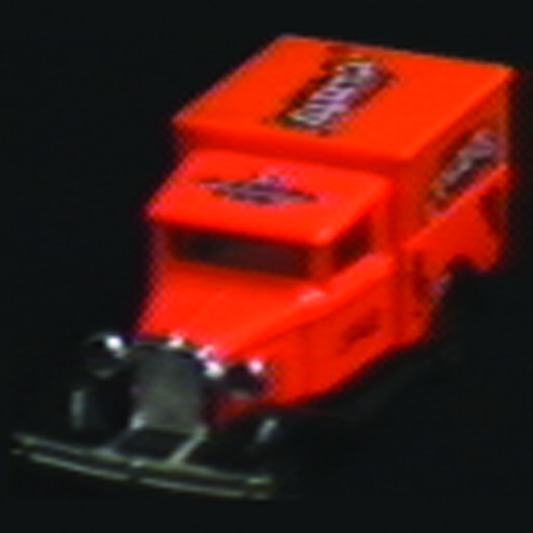
\includegraphics[width=0.2\linewidth]{figures/taxonomy/obj100__295.jpg}
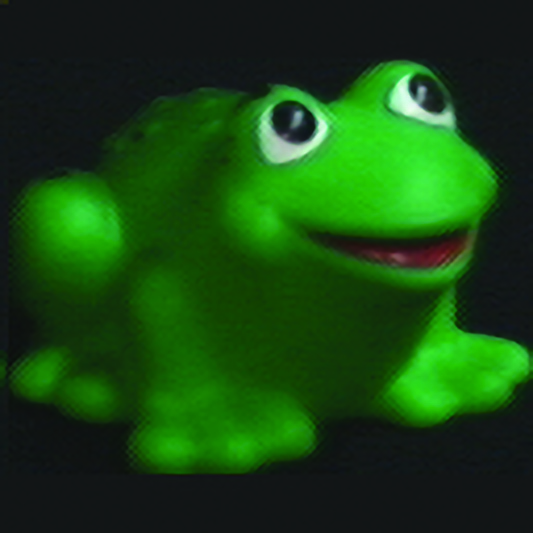
\includegraphics[width=0.2\linewidth]{figures/taxonomy/obj28__240.jpg}
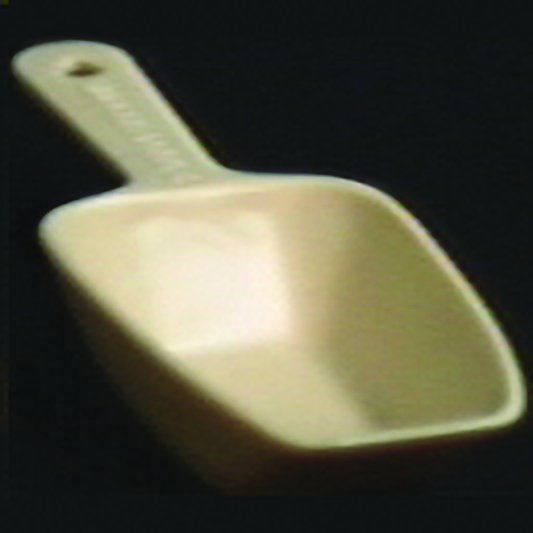
\includegraphics[width=0.2\linewidth]{figures/taxonomy/obj44__255.jpg}
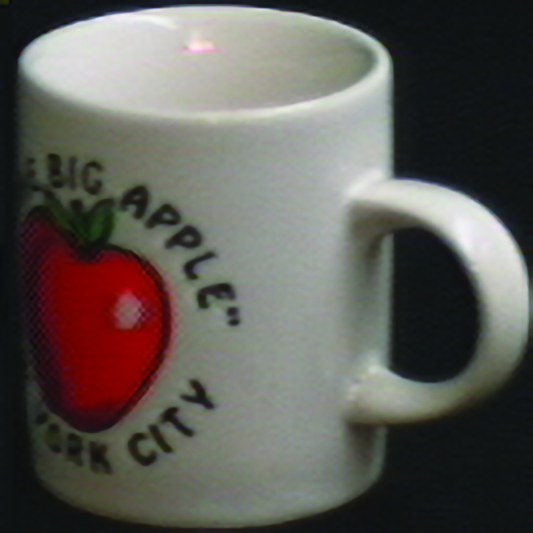
\includegraphics[width=0.2\linewidth]{figures/taxonomy/obj45__35.jpg}
}
}

The decade of 2010--2020 has been clearly dominated by learning-based methods using deep learning as the main framework in all areas of computer vision. 

\subsection{Learning-Based Vision}

%\reviewcomment{Unfinished. Text incomplete and missing references.}


While many previous perspectives on perception began with models about how perception might 
work, learning-based approaches take a different path. They rely on flexible architectures that incorporate as few hypothesis about perception as possible, and instead focus on data to learn to build the right model for perception.

Learning-based vision has its roots in the philosophical tradition of empiricism, which holds that knowledge about the world should be acquired by experience, rather than solely through reason (an approach known as rationalism). The modern day term for experience is ``data,'' and learning is really all about data. 



Learning derives vision algorithms by fitting functions to data. One way to think about it is that our goal is to ``program'' a vision algorithm and there are a few ways to do so (\fig{\ref{fig:taxonomy:programming_vs_learning}}). One way is to write the algorithm directly in Python code: first we will compare the intensity of this pixel and that pixel, then we will threshold about some such value, and so on. Another approach is to derive the algorithm as the rational thing to do given some underlying model of the world, for example, because overlapping objects generically produce contrast edges in the image, the optimal way to detect boundaries between objects is to look for such and such particular kind of contrast. The third approach --- the learning approach --- is to program algorithms via data: first collect a bunch of examples of inputs and the correct output, then fit a function that replicates these exemplar mappings from input to output.


\begin{figure}[t]
\centerline{
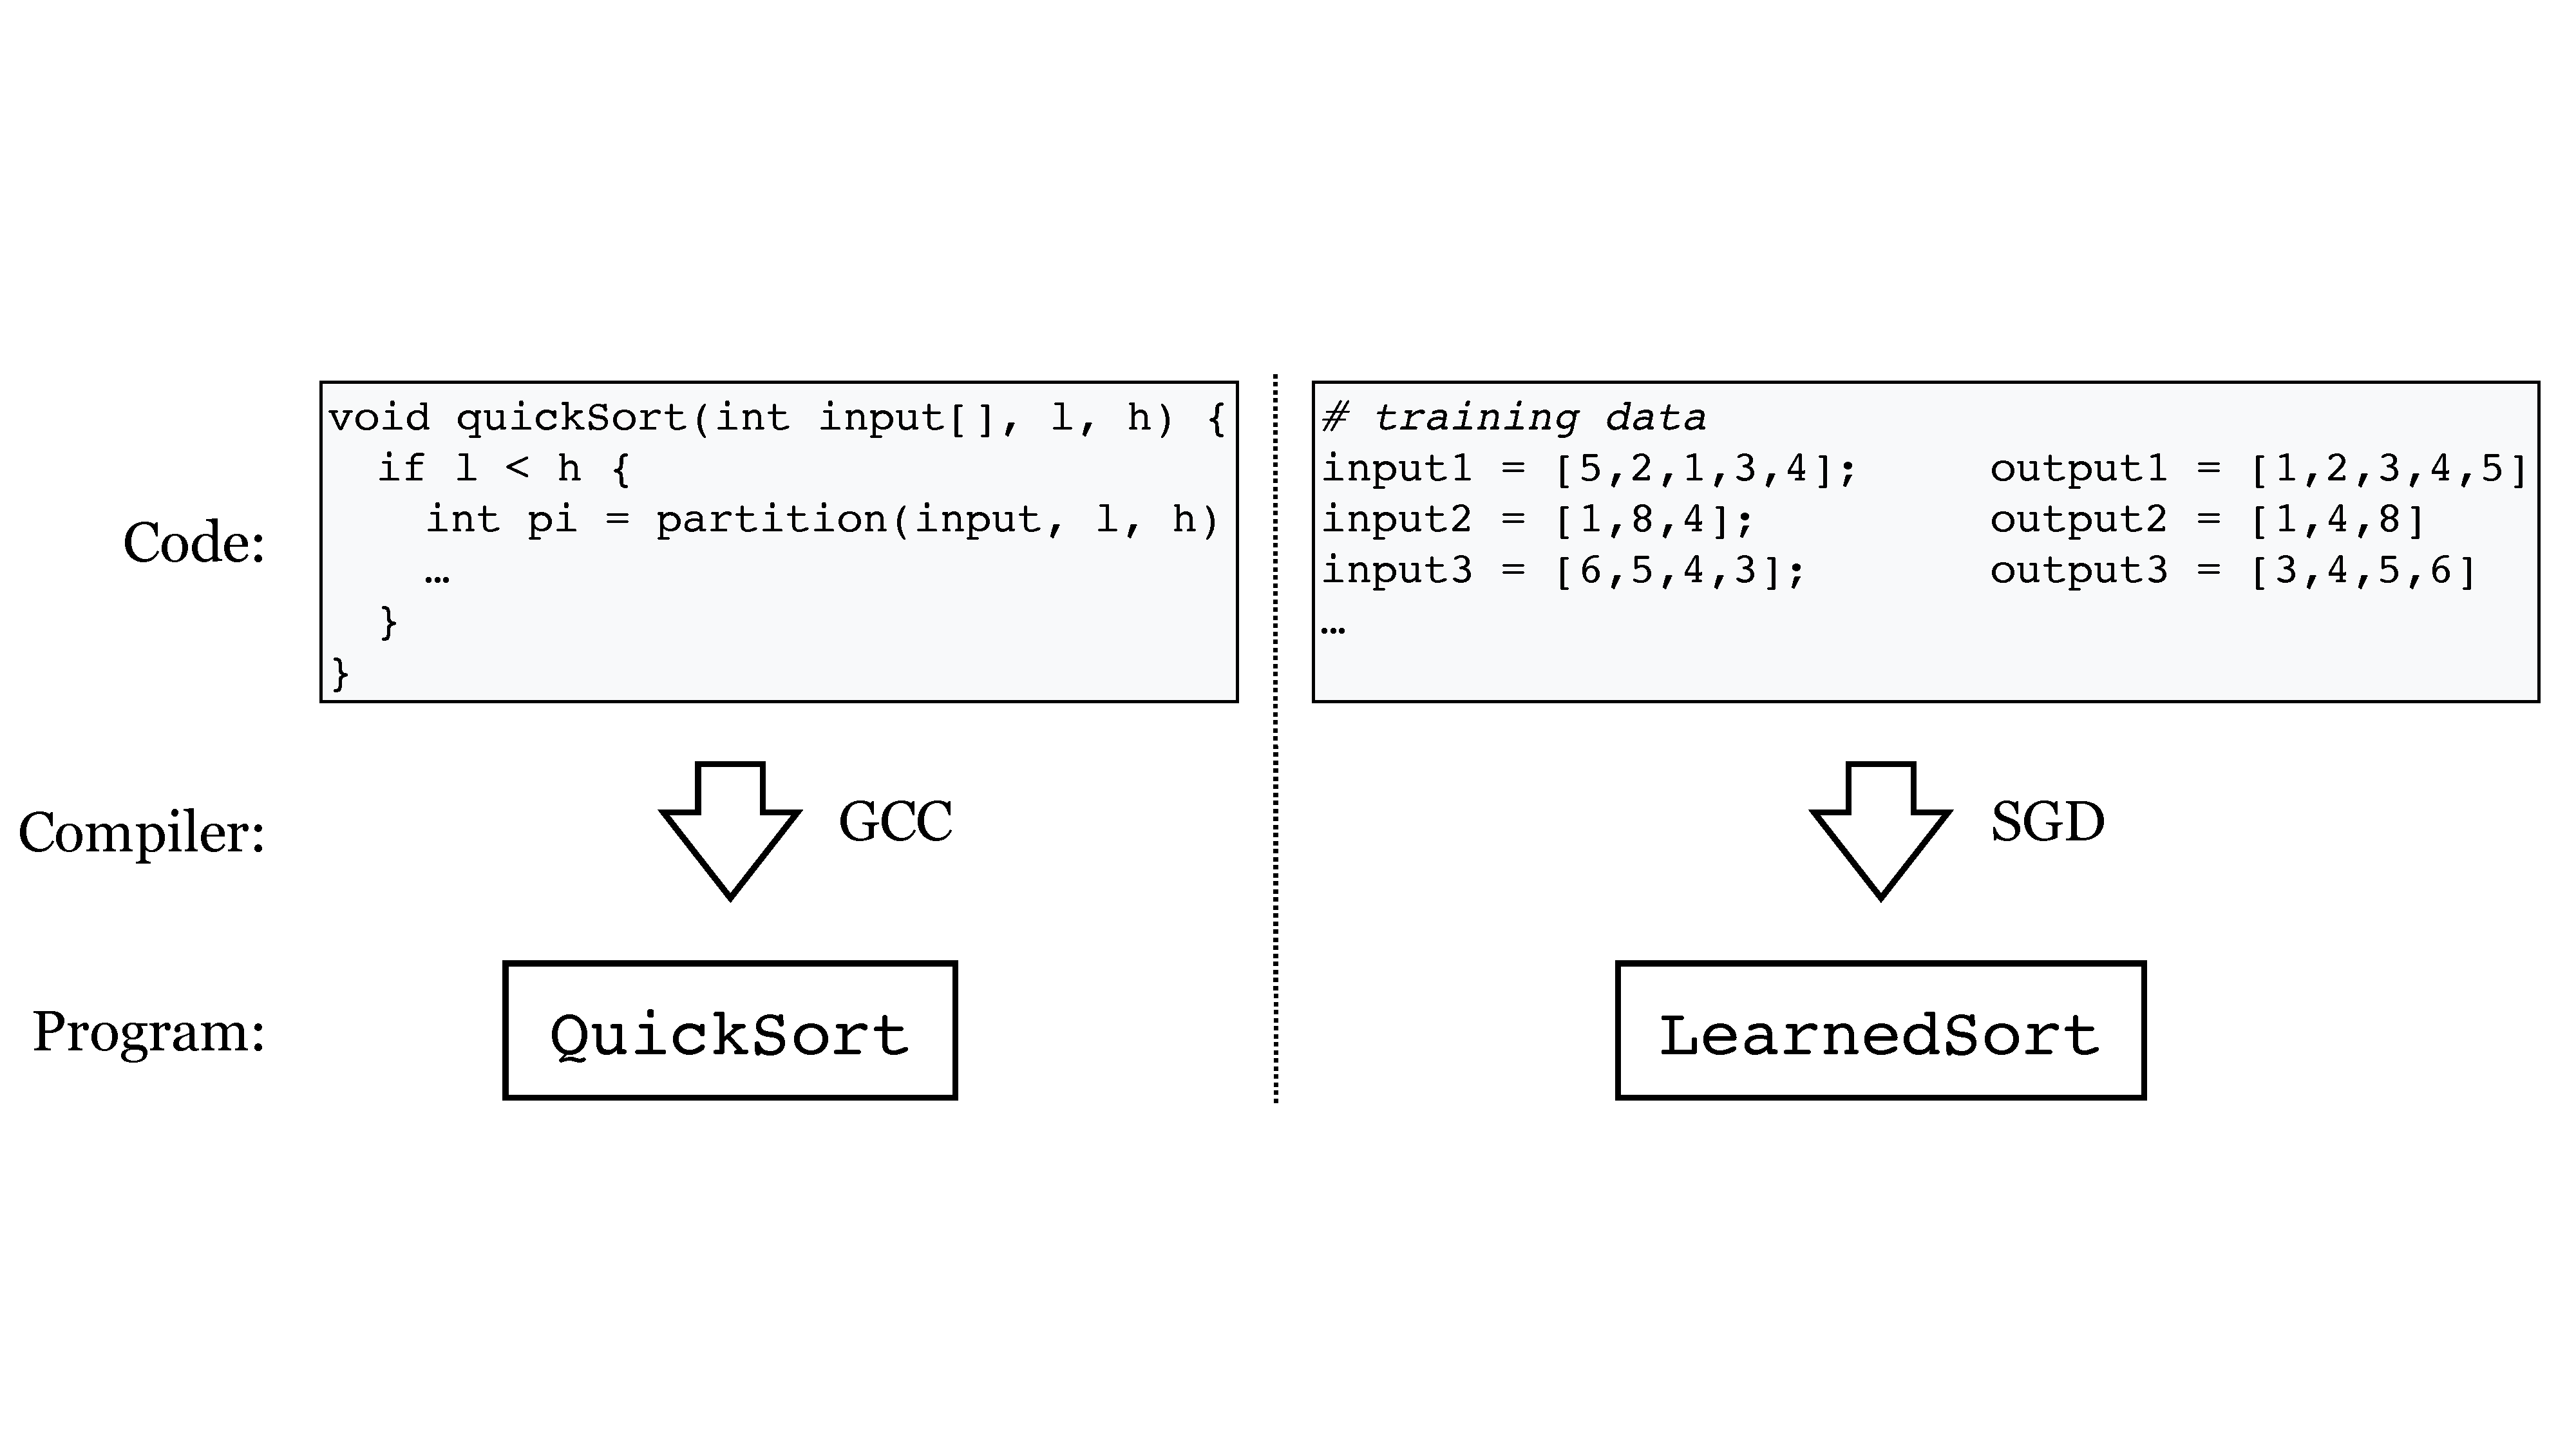
\includegraphics[width=1\linewidth]{figures/taxonomy/programming_vs_learning.pdf}
} 
\caption{Two ways of programming an algorithm. Left: traditional way, Right: the machine learning way. You will learn about the machine learning ``compiler'', called Stochastic Gradient Descent (SGD), in \chap{\ref{chapter:backpropagation}}.} 
\label{fig:taxonomy:programming_vs_learning}
\end{figure}


Learning algorithms have been a part of computer vision since the field's origins. In 1958, Frank Rosenblatt published one of the first formal learning algorithms, called the {\bf perceptron}\index{Perceptron}
learning algorithm, and showed that it can, in principle, learn to recognize certain simple visual patterns~\cite{rosenblatt1958perceptron}. 
The perceptron was also one of the first artificial neural nets, a computational model of biological brains. The ability of perceptrons to learn to solve recognition problems created an explosion of interest in neural nets. 

\marginnote{
Rosenblatt published the perceptron algorithm in the journal \booktitle{Psychological Review} in 1958. This is a nice example of the interdisciplinary nature of the AI field in its origins.
}

Interest in neural nets has since gone through a series of ebbs and flows (\fig{\ref{fig:taxonomy:neural_net_enthusiam}}). Note that these cycles have partially lined up with interest in learning algorithms more generally, but there have also been phases where interest in neural nets was low but interest in other learning algorithms was high.

\begin{figure}[t]
\centerline{
\includegraphics[width=0.7\linewidth]{figures/taxonomy/neural_net_enthusiasm.eps}
} 
\caption{Enthusiasm for neural nets has gone up and down over time, with a period of roughly 25 years. What will happen next?} 
\label{fig:taxonomy:neural_net_enthusiam}
\end{figure}


In 1969, Marvin Minsky and Seymour Papert published a book titled \booktitle{Perceptrons: an introduction to computational geometry}~\cite{marvin1969perceptrons}. You might think this would be a book that would increase the excitement around perceptrons, but in fact it largely killed it. Minsky and Papert showed that perceptrons are incapable of learning basic logical operations. Clearly then, perceptrons could not be the basis of intelligence.

It wasn't until the 1980s that interest in learning algorithms, and neural nets in particular, began to surge again. The reason was because researchers showed that perceptrons could be stacked to create systems capable of complex operations, including logic. These systems were the precursors to the {\bf deep learning} systems that are dominate today. In this decade, several architectures specific to vision were also introduced, including Kunihiko Fukushima's \booktitle{neocognitron}\index{Neocognitron}, which was a precursor to modern convolutional neural networks~\cite{fukushima1980neocognitron}. In 1989, Yann LeCun et al. showed how these kinds of networks can be efficiently trained \cite{lecun1989backpropagation} and their system was put into use for recognizing handwritten digits by the US Postal Service.


One of the peaks of neural network research in the 1980s was the publication of \booktitle{Parallel Distributed Processing} by David Rumelhart and Jay McClelland~\cite{Rumelhart86}. This book mixed the neuroscience of the brain with computational models of distributed processing in artificial networks. 

\marginnote{\booktitle{Parallel Distributed Processing}~\cite{Rumelhart86} cover:
\\[6pt]
\centerline{
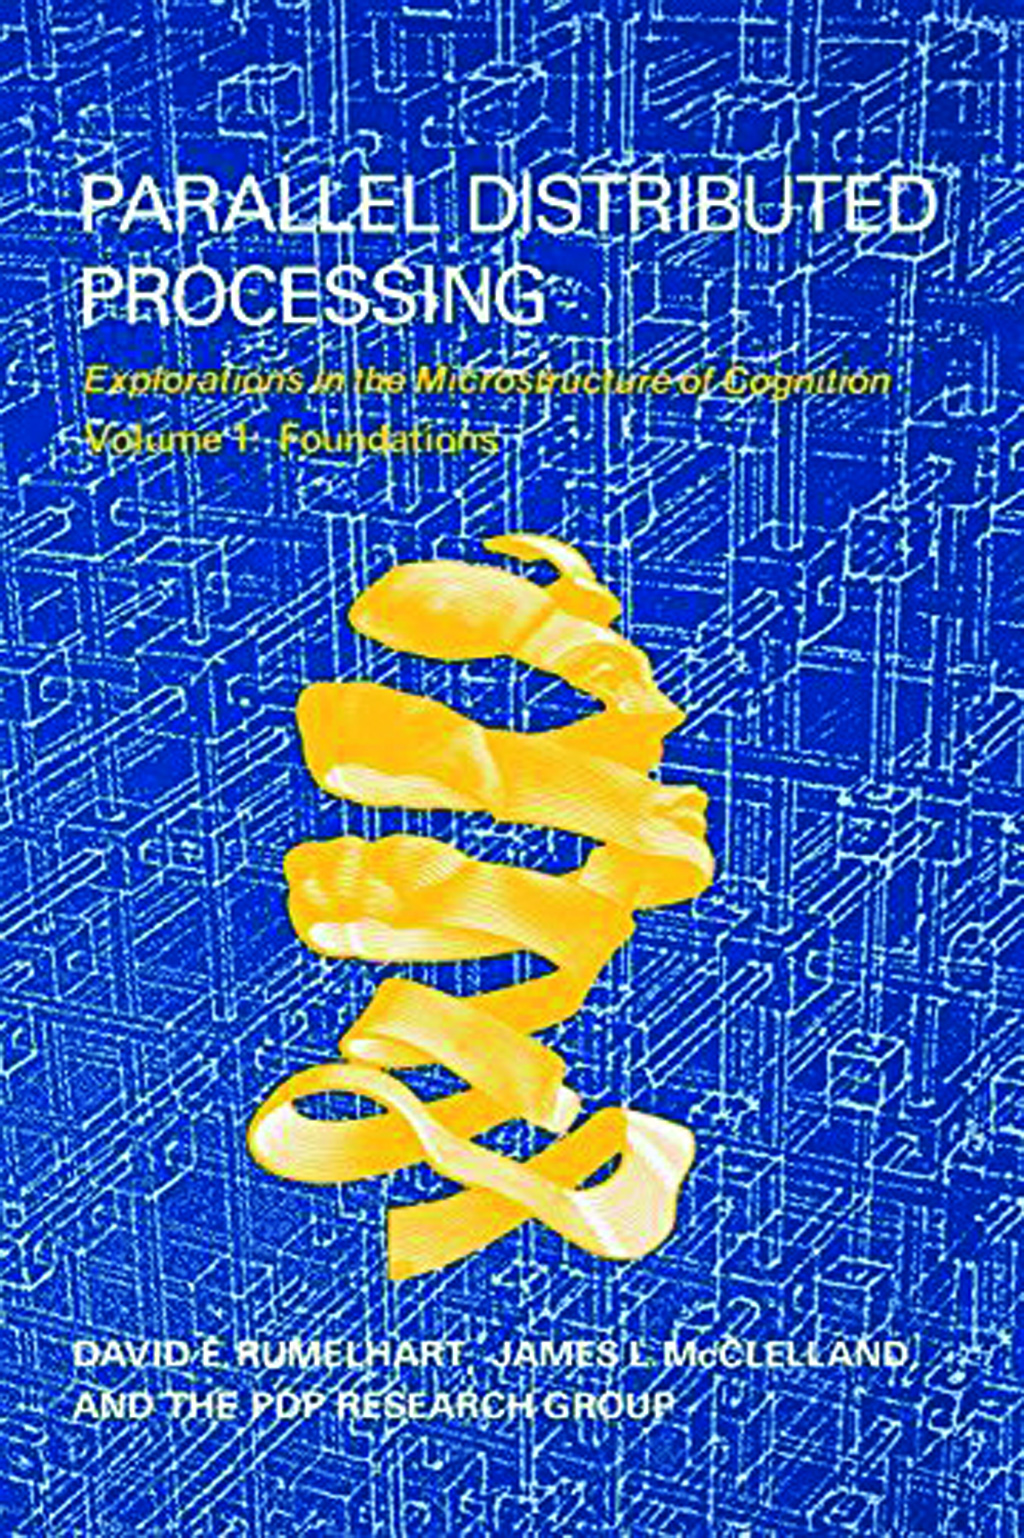
\includegraphics[width=.35\linewidth]{figures/taxonomy/pdp_cover.jpg}}
}[-.8in]

Unfortunately, however, at that time we did not have the compute and data necessary to make these systems really work, and interest waned during the 1990s. By the year 2000, the field of AI as a whole was firmly in a ``winter''; the promises of the 1980s had failed to materialize and the study of learning algorithms continued on without much fanfare in just a few corners of academia. Nonetheless, several major advances did occur in the relative quiet of the 1990s and early 2000s. 
For example, in 2001, Paul Viola and Michael Jones published a method that used a simple learning algorithm called {\bf boosting} to detect faces in photos~\cite{Viola01}. 
\marginnote{Face detection example from \cite{Viola01}:
\\[6pt]
\centerline{
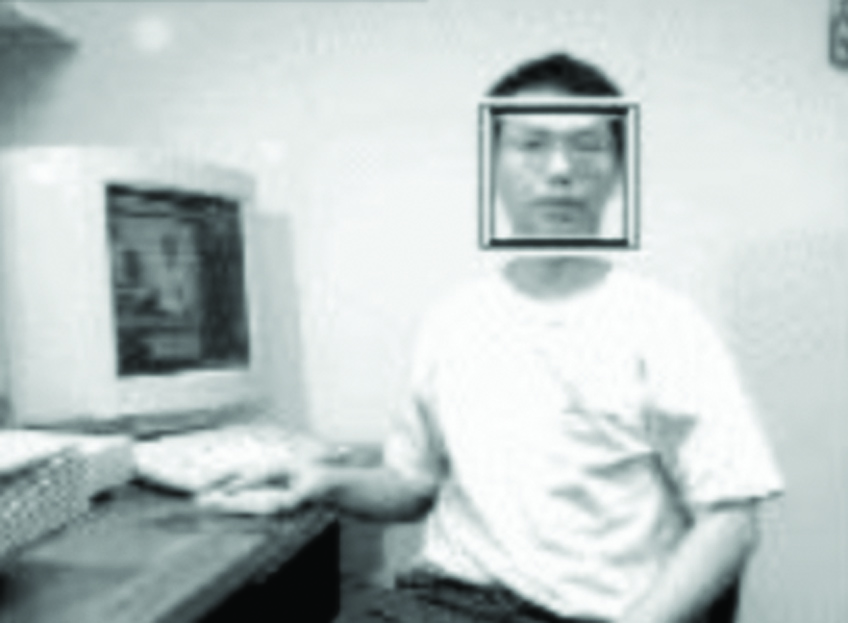
\includegraphics[width=.4\linewidth]{figures/taxonomy/viola_jones_example.jpg}}
}[-1.25in]
This method outperformed the complicated hand-engineered face detectors of the time in terms of computational efficiency and detection rate, and even became a popular algorithm used in consumer cameras.



The 2000s were a decade where learning returned to the foreground. One common pattern was to take the best hand-engineered features and feed them as input to a shallow learning machine, such as a support vector machine~\cite{cortes1995support}. Gradually more and more of the vision pipeline was replaced with learned modules. Finally, in 2012, a deep neural net called AlexNet dramatically outperformed all existing methods for image classification, and did so with a system that used learning \textbf{end-to-end} (for each processing stage from the input pixels to the output predictions)~\cite{krizhevsky2012imagenet}. This event has come to be called the ``ImageNet Moment'' since AlexNet's dramatic performance was first demonstrated at the 2012 ImageNet competition~\cite{russakovsky2015imagenet}.
\marginnote{WordNet is an electronic dictionary used to define word hierarchies \cite{Fellbaum1998}:
\\[6pt]
\centerline{
\includegraphics[width=.4\linewidth]{figures/taxonomy/exampleTree12.eps}
}
}[-.8in]
The ImageNet moment was a watershed for learning-based vision and for neural networks. In the few years after 2012, learning became the key ingredient in almost all research on computer vision. As of the 2020s, it is hard to find any computer vision system that does not use deep learning somewhere in its pipeline.

It may seem like learning-based vision is very different than other approaches, but actually it is similar in many ways. The study of vision consists of the structure of the input, the structure of the output, and the mapping between the two. Learning-based vision does not fundamentally change any of these: the input and target output are the same as before, and the mapping is remarkably similar as in other approaches. The big difference with learning-based vision is how you \textit{find} the mapping. In this sense, learners are just like a new kind of vision scientist: they play the same role as the humans who, in previous eras, sat down and thought deeply to determine the way vision works.


%-- let the data determine the solution -- which stands in contrast to philosophical schools based on logic / deduction.


%Learning-based vision is actually not so different than other approaches, except that the vision algorithms are ``programmed" by a machine learner rather than by a human. 
In this book we will see that very often machine learners come up with similar vision algorithms as were previously designed by humans. But in many ways machine learners are also more powerful than human designers, and machine learned algorithms have now far exceeded those designed by humans in terms of raw performance.



%1980 - Kunihiko Fukushima; neocognitron

%2001 - Viola and Jones

%2012 - deep learning


%the communities in cognition, neuroscience and computer vision got separated 

%Graph of enthusiam for neural nets over time.


%There is now a trend into building general vision systems 

%And hopefully soon, the areas of cognition, neuroscience and computer vision will work together again to advance our understanding of natural and artificial intelligence. 


%Do the learning approaches overestimate the importance of learning and undervalue the importance of model-driven representations? 


 
\section{What's Next?}


In a span of more than 2000 years, from the Greeks' extramission theories of vision to the understanding of the neural mechanisms and the engineering of computer vision systems, we have come a long way in our understanding of the nature of perception. 
Each step during the evolution of vision theories revealed important aspects of perception ignored by the previous theories. What theories will come next? What is missing now? Certainly, many things. For instance, we are missing visual common sense (now powered by large language models), integration with other perceptual systems, and, most importantly, a theory of embodied perception. And those are just the most obvious. There might be many other steps missing that we are not smart enough to see from where we are standing right now. 



\section{Concluding Remarks}

The goal of this chapter was to define the topic of computer vision by placing it inside its historical context. We believe that any researcher of computer vision would benefit by studying vision from an interdisciplinary perspective as it will provide a solid basis for creativity, technical depth, and an understanding of its societal impact. We hope this chapter also inspires students to learn more about this fascinating field and to get excited by its potential.


